\chapter{Working Out Layout and Sketches with AI}
\usetikzlibrary{decorations.pathreplacing}

Lin Yue, a doctoral student in molecular biology, is preparing her dissertation proposal and drafting the introduction to a review on genome editing. She needs Figure 1: a full-width overview schematic showing life-science peers and reviewers how \emph{Streptococcus pyogenes} Cas9 (SpCas9), guided by a single guide RNA (sgRNA), recognizes a protospacer-adjacent motif (PAM) and cleaves double-stranded DNA, and how non-homologous end joining (NHEJ) and homology-directed repair (HDR) yield distinct editing outcomes.

She opens an image generator and enters a single prompt: ``Draw a professional, visually striking overview figure of the CRISPR--Cas9 genome editing mechanism suitable for a top journal.'' Seconds later, the tool returns a glossy landscape illustration: inside a three-dimensional dark-blue cell nucleus, glowing cyan scissors slice through a twisted DNA helix, while the four corners hold a ribbon-like RNA strand, a glowing ``PAM'' badge, and two short DNA fragments—one cracked and one patched with color.

Impressed by the surface polish, Lin Yue drops the image into her slides. Her advisor looks at the screen for five seconds and asks: ``Where am I supposed to start reading this figure?''

Lin Yue hesitates. Her advisor points out the visual traps: a reader's eye goes straight to the largest, brightest element at the center—the glowing scissors—even though cleavage is the third step. After the scissors, should the eye move to the top-left corner for the RNA, or to the bottom-right corner for the repaired DNA? Worse, the two repaired DNA fragments sit in the bottom-left and bottom-right corners with no connecting arrows and no shared baseline. How can a reader tell that they represent parallel repair choices branching from one break, rather than sequential steps?

This first draft fails not from poor rendering, but because the author clicked ``Generate'' before deciding the reader's entry point and eye path. Without a spatial skeleton, an image model defaults to decorative symmetry—placing a dramatic object at the center and scattering the remaining nouns into the corners. This chapter moves layout exploration and sketching ahead of rendering, addressing five questions: how to control reading order via ``entry--path--endpoint,'' how to decide what belongs in one panel, how to draw three distinct layout sketches from a single brief, how to generate and evaluate candidates in \scidraw{}, and how to revise with one verifiable goal per pass.

\section{Reading Order Comes Before Rendering}

When readers encounter an overview figure, they do not scan it word by word like text. In the first few seconds, vision follows instinct: the eye lands on the heaviest visual anchor and follows geometric cues across the canvas (Wong, 2011c; Rougier et al., 2014). If a figure cannot show ``where to start, where to go, and where to stop'' within five seconds, even finely rendered molecules will impede comprehension.

Before sketching or prompting, plan the viewer's trajectory by answering three questions:

\begin{itemize}
\item \textbf{First, where is the entry point?} The first fixation lands on the region of greatest visual weight—usually the largest shape, strongest luminance or color contrast, most isolated element, or conventional starting corner (top-left or far-left in horizontal layouts). Without a clear anchor, or when three or four equally prominent blobs compete for attention, the reader hesitates immediately.
\item \textbf{Second, how does the path move?} Once inside the frame, the eye needs geometric guides. Explicit guides include unidirectional arrows and step numbers (1, 2, 3, and so on); implicit guides include shared horizontal or vertical alignment baselines, continuous white-space channels, and natural left-to-right or top-to-bottom progression.
\item \textbf{Third, where does the path end?} The final resting point should hold the core scientific takeaway. Inflating upstream background components while cramping the final comparison or repair outcomes into a corner inverts the visual hierarchy, reducing the main message to a footnote.
\end{itemize}

\begin{figure}[htbp]\centering
\resizebox{\linewidth}{!}{% FIG ch03-01 reading order (English)
\begin{tikzpicture}[
  x=1mm, y=1mm,
  font=\sffamily\footnotesize,
  panel/.style={draw=BookInk!40, line width=0.3pt, rounded corners=1pt},
  block/.style={
    rounded corners=2pt, draw=black!60, fill=black!5,
    minimum size=7mm, inner sep=0pt, font=\sffamily\footnotesize,
  },
  eye/.style={line width=4pt, draw=blue!50, opacity=0.35, rounded corners=2pt},
  paneltitle/.style={font=\sffamily\scriptsize, text=BookInk, align=center},
]
  \def\pw{50}\def\ph{35}
  \begin{scope}[shift={(0,42)}]
    \draw[panel] (0,0) rectangle (\pw,\ph);
    \node[paneltitle, anchor=north] at (0.5*\pw,\ph+2.5) {(a) Linear};
  \end{scope}
  \begin{scope}[shift={(54,42)}]
    \draw[panel] (0,0) rectangle (\pw,\ph);
    \node[paneltitle, anchor=north] at (0.5*\pw,\ph+2.5) {(b) Hub};
  \end{scope}
  \begin{scope}[shift={(108,42)}]
    \draw[panel] (0,0) rectangle (\pw,\ph);
    \node[paneltitle, anchor=north] at (0.5*\pw,\ph+2.5) {(c) Two-branch};
  \end{scope}
  \begin{scope}[shift={(0,42)}]
    \foreach \i/\x in {1/8,2/18,3/28,4/38,5/42} {
      \node[block] at (\x,17.5) {\i};
    }
    \draw[eye] (6,22) .. controls (15,26) and (35,26) .. (44,22);
    \foreach \i/\xa/\xb in {1/11/15,2/21/25,3/31/35,4/41/45} {
      \draw[-{Stealth[length=1.2mm]}, draw=BookInk!35, thin] (\xa,17.5) -- (\xb,17.5);
    }
  \end{scope}
  \begin{scope}[shift={(54,42)}]
    \node[block] at (25,17.5) {3};
    \node[block, minimum size=5.5mm] at (8,28) {1};
    \node[block, minimum size=5.5mm] at (42,28) {2};
    \node[block, minimum size=5.5mm] at (8,7) {4};
    \node[block, minimum size=5.5mm] at (42,7) {5};
    \draw[eye, blue!50] (25,20) .. controls (32,26) .. (42,28);
    \draw[eye, orange!70!black, opacity=0.35] (25,20) .. controls (18,26) .. (8,28);
    \draw[eye, blue!50] (25,15) .. controls (32,8) .. (42,7);
    \node[font=\Large, text=BookInk!60] at (32,17) {?};
  \end{scope}
  \begin{scope}[shift={(108,42)}]
    \foreach \i/\x in {1/10,2/25,3/40} {
      \node[block, minimum size=6mm] at (\x,28) {\i};
    }
    \node[block, minimum size=6mm] at (25,12) {4};
    \node[block, minimum size=6mm] at (25,5) {5};
    \draw[-{Stealth[length=1mm]}, draw=BookInk!35, thin] (13,28) -- (22,28);
    \draw[-{Stealth[length=1mm]}, draw=BookInk!35, thin] (28,28) -- (37,28);
    \draw[-{Stealth[length=1mm]}, draw=BookInk!35, thin] (40,26) -- (40,20) -- (25,20) -- (25,15);
    \draw[-{Stealth[length=1mm]}, draw=BookInk!35, thin] (25,20) -- (25,8);
    \draw[eye] (8,30) .. controls (18,32) .. (38,30) .. controls (42,22) .. (25,14);
    \draw[eye] (25,14) -- (25,6);
  \end{scope}
  \def\bw{38}\def\bh{22}
  \foreach \i/\x/\title in {
    1/0/Proximity, 2/42/Alignment, 3/84/Enclosure, 4/126/Hierarchy} {
    \begin{scope}[shift={(\x,0)}]
      \draw[panel] (0,0) rectangle (\bw,\bh);
      \node[paneltitle, anchor=north] at (0.5*\bw,-2.5) {\title};
    \end{scope}
  }
  \begin{scope}[shift={(0,0)}]
    \foreach \x in {6,10,14} {\fill[BookInk] (\x,14) circle (0.9mm);}
    \foreach \x in {26,30,34} {\fill[BookInk] (\x,14) circle (0.9mm);}
  \end{scope}
  \begin{scope}[shift={(42,0)}]
    \draw[fill=BookInk!15, draw=BookInk!50] (4,6) rectangle (16,18);
    \draw[fill=BookInk!15, draw=BookInk!50] (4,6) rectangle (14,18);
    \node[font=\scriptsize, anchor=west] at (18,12) {Aligned};
    \node[font=\scriptsize, anchor=west, text=BookInk!55] at (18,7) {Misaligned};
  \end{scope}
  \begin{scope}[shift={(84,0)}]
    \draw[fill=BookRule!40, rounded corners=2pt] (3,5) rectangle (35,19);
    \foreach \x in {10,19,28} {
      \draw[fill=BookPale, draw=BookInk!40, rounded corners=1pt] (\x-3,9) rectangle (\x+3,15);
    }
  \end{scope}
  \begin{scope}[shift={(126,0)}]
    \draw[fill=BookInk!25, draw=BookInk!60, rounded corners=2pt] (14,6) rectangle (26,18);
    \foreach \x/\y in {6/16,6/10,32/16,32/10} {
      \draw[fill=BookInk!8, draw=BookInk!45, rounded corners=1pt] (\x-2.5,\y-2) rectangle (\x+2.5,\y+2);
    }
  \end{scope}
\end{tikzpicture}
}
\caption{Layout decides reading order. Top: the same five elements arranged in three structures; translucent curves show the most likely eye path. The hub layout has no single entry point, so readers may take different routes. Bottom: four basic ways to control hierarchy and grouping.}\label{fig:ch03-01}
\end{figure}

The upper row of Figure~\ref{fig:ch03-01} shows how arranging the same five sequential nodes (1 to 5) into three structures alters the eye path. In the \textbf{linear layout} (Figure~\ref{fig:ch03-01}a), five rounded blocks sit in a single row linked by gray arrows; the translucent blue curve traces an unambiguous left-to-right trajectory from node 1 to node 5, ideal for unbranched sequences.

Now consider the \textbf{hub layout} (Figure~\ref{fig:ch03-01}b), where node 3 sits enlarged at the center and nodes 1, 2, 4, and 5 occupy the four corners. While common in mind maps, this structure disrupts sequential processes. As the conflicting blue and orange curves show, readers take different routes: some start at the large central node 3 and jump toward 2 or 5; others start by habit at top-left node 1, pass through 3, and stall—marked by the question mark—unsure whether to go to the upper right or lower left. Without a unique entry point, readers must guess the sequence.

Figure~\ref{fig:ch03-01}c shows a \textbf{two-branch layout} suited for ``shared upstream pathway, two alternative outcomes.'' Nodes 1, 2, and 3 form a compact top row from left to right; from node 3, a downward arrow splits into two parallel branches feeding vertically stacked nodes 4 and 5. The eye scans the upstream sequence horizontally, follows the fork downward, and immediately reads 4 and 5 as parallel outcomes from node 3.

With the skeleton in place, four visual mechanisms govern internal order (Figure~\ref{fig:ch03-01}, bottom row), drawing on Gestalt perception (Wong, 2010a, 2010b) and visual hierarchy (Wong, 2011d):

\begin{enumerate}
\item \textbf{Proximity:} Nearby elements are grouped automatically. In the first bottom panel of Figure~\ref{fig:ch03-01}, six dots divide into two triplets solely through tight internal spacing and a wide central gap. In scientific figures, open background (negative space) is not wasted paper; it is the divider separating stages or complexes (Wong, 2011b). When a generator packs objects evenly across the canvas, losing proximity contrast makes the image look chaotic.
\item \textbf{Alignment:} Elements sharing a horizontal baseline or vertical left edge are read as comparable peers (Figure~\ref{fig:ch03-01}, second bottom panel). When comparing two DNA repair outcomes, aligning the left and right endpoints of both duplexes lets readers spot the central change instantly; staggered or unequal strands make readers wonder whether the offset implies biological truncation.
\item \textbf{Enclosure:} Framing elements inside a tinted box or thin rectangle is the strongest grouping cue (Figure~\ref{fig:ch03-01}, third bottom panel). When a repair pathway includes a cleaved substrate, an exogenous donor template, and a repaired duplex, enclosing the lane keeps the floating donor from being misassigned to the adjacent pathway.
\item \textbf{Hierarchy:} A figure should have only one center of primary visual weight (Figure~\ref{fig:ch03-01}, fourth bottom panel). Adding more bright colors only makes every object compete. Instead, combine \textbf{size, luminance contrast, and position}: give the main comparison the largest area and whitespace, reserve high-contrast accents for active changes (such as the PAM, indel scar, or inserted sequence), and mute invariant scaffolding in neutral gray.
\end{enumerate}

These four mechanisms reduce to one rule: \textbf{grouping is a scientific claim.} Objects placed close together, aligned on a baseline, enclosed in a frame, or given the same color will be read as scientifically related. Likewise, causal sequences should follow left-to-right or top-to-bottom reading direction, and parallel branches must share symmetrical geometry so options are not misread as sequential steps.

Before refining a draft, run three quick self-tests: (1) the \textbf{five-second test}—show the draft to a colleague unfamiliar with the brief for five seconds, hide it, and ask what they saw first and what the figure compares; (2) \textbf{finger tracing}—ask the colleague to trace their eye path with a finger, noting any pause or backtrack as a broken layout cue; and (3) the \textbf{half-scale grayscale check}—shrink the figure to 50\% of its print width (e.g., 87 mm for a 174 mm figure) in grayscale to confirm a single visual center and clear white-space channels.

\section{What Belongs in One Panel}

Once reading order is set, we must decide how much to include. The second common flaw in overview figures is overcrowding: trying to show plasmid or ribonucleoprotein (RNP) delivery across the cell membrane, nuclear pore entry, chromosome and nucleosome unwinding, a 3D Cas9 crystal structure with HNH and RuvC catalytic residues, repair factors (Ku70/80, DNA-PKcs, Ligase IV), microhomology-mediated end joining (MMEJ), off-target cleavage, and base editing—all inside one 174 mm panel. Cramming thirty multi-scale objects together makes both the overall pathway and the molecular geometry illegible.

The rule is simple: \textbf{one panel answers one core question; only elements that the reader must see simultaneously to follow the causal chain or compare outcomes belong in the same panel.}

Using the one-sentence template from Chapter 1, Lin Yue states the testable task for her Figure 1:

\begin{BookNote}
After viewing this figure, the reader should be able to understand \textbf{how a single guide RNA (sgRNA) directs Cas9 to recognize a target sequence adjacent to a PAM and generate a double-strand break, after which non-homologous end joining (NHEJ) and homology-directed repair (HDR) produce either imprecise small insertions/deletions or precise template-directed edits}, and be able to locate \textbf{the chronological order of events, the relative positions of the PAM and cleavage site, and the sequence-level difference between the two repair outcomes}.
\end{BookNote}

This overview reports no new experimental data; every relationship rests on established textbook and review consensus: Jinek et al.\ (2012) showed that SpCas9 is a dual-RNA- or sgRNA-guided endonuclease that requires a PAM on the non-target strand and uses HNH and RuvC-like domains to cleave the target and non-target strands, respectively; Ran et al.\ (2013) defined practical SpCas9 design rules, placing double-strand cleavage about 3 base pairs (bp) upstream of the $5'$-NGG-$3'$ PAM; Doudna and Charpentier (2014) and Hsu et al.\ (2014) summarized how Cas9 breaks route into NHEJ or HDR outcomes; and Chang et al.\ (2017) detailed the fidelity and mechanisms of NHEJ versus alternative end-joining pathways.

Before sketching, the author compiles these established facts into nine verifiable relationships (Table~\ref{tab:ch03-01-rel}, C1--C9).

\begin{table}[htbp]\centering\footnotesize
\setlength{\tabcolsep}{3pt}
\renewcommand{\arraystretch}{1.15}
\caption{Relationship table (C1--C9) for the CRISPR--Cas9 genome editing overview figure. All relationships represent established consensus; visual simplifications must be declared in the legend.}\label{tab:ch03-01-rel}
\begin{tabularx}{\linewidth}{@{}l>{\raggedright\arraybackslash}p{24mm}>{\raggedright\arraybackslash}p{24mm}>{\raggedright\arraybackslash}p{20mm}Y@{}}
\toprule
\textbf{\#} & \textbf{Source / Input} & \textbf{Target / Outcome} & \textbf{Relationship \& Status} & \textbf{Visual Simplification in This Figure} \\
\midrule
C1 & sgRNA (fused crRNA:tracrRNA strand) & Cas9 protein & Binds to form Cas9--sgRNA complex (Established) & Omit sgRNA secondary-structure details; draw as an orange strand with spacer and hairpin loop \\
C2 & Cas9--sgRNA complex & Genomic DNA PAM ($5'$-NGG-$3'$ for SpCas9) & Recognizes PAM (Established) & Omit 3D diffusion and 1D sliding search along DNA \\
C3 & sgRNA spacer ($\sim$20 nt) & Target DNA strand (complementary to spacer) & Base-pairs to form R-loop; non-target strand displaced (Established) & Omit stepwise zipping kinetics of R-loop formation \\
C4 & Spatial position of PAM & Non-target strand, immediately $3'$ of protospacer & Strand polarity and adjacency (Established) & Show as a yellow highlight in main panel; place exact $5'\rightarrow 3'$ polarity in the inset \\
C5 & Cas9 (HNH and RuvC-like domains) & Both strands cut $\sim$3 bp upstream of PAM & Generates double-strand break, mostly blunt (Established) & Do not separate domains in main panel; distinguish HNH and RuvC in the inset \\
C6 & Double-strand break & NHEJ (non-homologous end joining) & Template-free repair route (Established) & Omit Ku70/80, DNA-PKcs, Ligase IV; omit alternative end joining (MMEJ) \\
C7 & NHEJ repair process & Small insertions or deletions (indels) may arise at break site & Outcome; can cause frameshift in coding exons (Established) & Use ``may''; NHEJ can also rejoin ends accurately, leading to recleavage cycles omitted here \\
C8 & Double-strand break + exogenous donor (with homology arms) & HDR (homology-directed repair) & Template-dependent repair route (Established) & Omit end resection and strand invasion intermediates \\
C9 & HDR repair process & Precise change copied from donor (insertion or replacement) & Outcome; lower frequency than NHEJ in most cells (Established) & Give no efficiency numbers; note lower frequency and S/G2 preference in legend only \\
\bottomrule
\end{tabularx}
\end{table}

Two nuances in Table~\ref{tab:ch03-01-rel} merit care. First, C7 states that indels \emph{may} arise at the break site rather than calling NHEJ invariably error-prone. As Chang et al.\ (2017) note, canonical NHEJ ligates compatible ends with high fidelity; in genome editing, indels accumulate because accurate rejoining restores the intact target and PAM, allowing persistent Cas9--sgRNA to recleave until an indel mutates the site. Although the diagram omits this recleavage loop for simplicity, the text and legend must retain ``may.'' Second, in C9, because HDR efficiency depends on cell type, cell-cycle phase (mainly S/G2), and donor design, the figure omits detached percentage numbers.

Cross-checking the task statement against Table~\ref{tab:ch03-01-rel} divides the material into three streams:

\begin{itemize}
\item \textbf{Stream 1: Keep in the main overview panel.} The main panel shows ``who acts, where, in what order, and with what two outcomes,'' retaining eight core objects: bilobed Cas9 silhouette, orange sgRNA, ladder-like double-stranded DNA, yellow PAM block, double-strand break gap, short double-stranded donor template (dark-gray homology arms with a teal central segment), NHEJ outcome DNA (with a reddish-purple indel mark), and HDR outcome DNA (with a teal inserted segment).
\item \textbf{Stream 2: Move to a detail inset.} Locating ``the relative positions of the PAM and cleavage site'' requires exact molecular geometry: antiparallel $5'\rightarrow 3'$ strands, the $5'$-NGG-$3'$ PAM on the non-target strand immediately $3'$ of the protospacer, the $\sim$20-nt sgRNA spacer paired with the target strand, cleavage $\sim$3 bp upstream of the PAM, and HNH cutting the target strand while RuvC cuts the non-target strand. Putting this in an inset keeps the main canvas clean while making base-level geometry explicit.
\item \textbf{Stream 3: Omit and declare in the legend.} Cells, nuclei, chromosomes, delivery vehicles (plasmids, RNPs, viruses), 3D Cas9 structure, repair enzymes, alternative end joining, off-target cuts, base or prime editing, and efficiency numbers are omitted and listed at the end of the legend.
\end{itemize}

\begin{figure}[htbp]\centering
% FIG ch03-07 PAM inset (English)
\begin{tikzpicture}[
  x=1mm, y=1mm,
  font=\sffamily\scriptsize,
  text=BookInk,
]
  \node[anchor=east] at (-2, 21.2) {Non-target strand};
  \node[anchor=east] at (-2, 7.2) {Target strand};
  \node at (6, 23.6) {5$'$};
  \node at (54.5, 23.6) {3$'$};
  \node at (55.5, 4.4) {5$'$};
  \node at (6, 4.4) {3$'$};

  \foreach \i in {0,...,19} {
    \pgfmathsetmacro{\x}{6+\i*2.4}
    \draw[draw=BookInk!50, fill=white] (\x,20) rectangle (\x+2.4,22.4);
  }
  \foreach \i in {0,1,2} {
    \pgfmathsetmacro{\x}{6+(17+\i)*2.4}
    \draw[draw=BookInk!50, fill=yellow!70] (\x,20) rectangle (\x+2.4,22.4);
  }
  \node[anchor=west, text=BookInk!80] at (6+17*2.4, 28.2) {PAM (NGG)};

  \foreach \i in {0,...,19} {
    \pgfmathsetmacro{\x}{6+\i*2.4}
    \draw[draw=BookInk!50, fill=white] (\x,6) rectangle (\x+2.4,8.4);
  }
  \foreach \i in {0,...,19} {
    \pgfmathsetmacro{\x}{6+\i*2.4}
    \draw[BookInk!35, thin] (\x+1.2,8.4) -- (\x+1.2,11.6);
    \draw[draw=orange!80!black, fill=orange!25, line width=1pt]
      (\x,4) rectangle (\x+2.4,6.4);
  }
  \draw[orange!80!black, line width=0.8pt]
    (6+19*2.4+2.4, 5) .. controls (6+21*2.4, 8) .. (6+21*2.4, 12)
    .. controls (6+21*2.4, 14) .. (6+19*2.4, 14);

  \node[anchor=west] at (6, 0.5) {sgRNA spacer};
  \pgfmathsetmacro{\cx}{6+16.5*2.4+1.2}
  \fill[black] (\cx,20) -- (\cx-0.8,21.2) -- (\cx+0.8,21.2) -- cycle;
  \fill[black] (\cx,6) -- (\cx-0.8,4.8) -- (\cx+0.8,4.8) -- cycle;
  \node[anchor=west] at (6+17.5*2.4, 13) {Cleavage site};
  \node[anchor=west, font=\scriptsize] at (6+16*2.4, 17) {RuvC};
  \node[anchor=west, font=\scriptsize] at (6+16*2.4, 3) {HNH};

  \draw[decorate, decoration={brace, amplitude=3pt}] (6, 15.5) -- (6+20*2.4, 15.5)
    node[midway, above=4pt] {$\sim$20 nt};
  \draw[decorate, decoration={brace, amplitude=2pt, mirror}] (6+16*2.4, 22.5) -- (6+17*2.4, 22.5)
    node[midway, below=2pt] {3 bp};
\end{tikzpicture}

\caption{Positions of the PAM and the cleavage site (SpCas9). The sgRNA spacer pairs with the target strand; the PAM ($5'$-NGG-$3'$) lies on the non-target strand immediately $3'$ of the protospacer. Both strands are cut about 3 bp upstream of the PAM, the target strand by the HNH domain and the non-target strand by the RuvC-like domain. Schematic; lengths not to scale.}\label{fig:ch03-07}
\end{figure}

Extracting the inset also reflects a critical tool-selection rule: \textbf{exact geometric relationships (strand polarity, which strand carries the PAM, and cut-site distance) should never be left to an image generation model; they must be drawn with deterministic tools.} Image models do not understand antiparallel nucleic acid rules and routinely place $5'$ and $3'$ on the same end, put the PAM on the wrong strand, or cut far from the PAM.

Figure~\ref{fig:ch03-07} shows the deterministic TikZ inset: the upper non-target strand runs $5'\rightarrow 3'$ left to right, with three yellow boxes at the $3'$ end of the 20-box protospacer labeled ``PAM (NGG)''; the lower target strand runs $3'\rightarrow 5'$ left to right; beneath it, the 20-box orange sgRNA spacer pairs box-for-box via vertical ticks and ends in a right-hand hairpin loop. Two black triangles mark the cleavage site between the third and fourth boxes upstream of the PAM (3 bp upstream), labeled ``RuvC'' on the non-target strand and ``HNH'' on the target strand (Jinek et al., 2012). In Section 6, this inset will be embedded directly into the upper-right corner of the final overview figure.

\section{From Words to Sketches: Draw Three Skeletons First}

In the \scidraw{} scientific figure workflow guide (\sdtool{figure-workflow}), we select the ``Mechanism and workflow figures'' route, replace the default brief with the text below, and download a local copy (shared across all three candidates, changing only the sketch):

\begin{Prompt}
[Use & Audience] Figure 1 overview schematic for a thesis proposal and review introduction; double-column width 174 mm by ~110 mm high. Audience: life-science peers and reviewers familiar with molecular biology basics.
[Goal] Show in order: sgRNA binds Cas9 -> complex recognizes PAM on DNA and pairs spacer with target strand -> cleaves both strands upstream of PAM to form a double-strand break -> two repair routes (NHEJ: template-free, may leave small indels; HDR: uses donor template for a precise edit). Main message: "One break, two repair pathways, two outcomes."
[Materials] Textbook and review consensus (Jinek 2012; Doudna & Charpentier 2014; Hsu, Lander & Zhang 2014; Ran et al. 2013). No experimental data.
[Objects] Cas9 (rounded bilobed silhouette); sgRNA (RNA strand with spacer and hairpin); genomic DNA (parallel lines with rungs); PAM (short highlight on DNA); double-strand break (gap across both strands); donor template (short dsDNA with homology arms and central insert); two repaired DNAs (NHEJ outcome, HDR outcome).
[Relationships] Follow C1-C9. Solid arrows between steps; split arrow after break into NHEJ and HDR; donor only in HDR lane aligned with the break.
[Layout] Follow attached sketch: A (linear), B (hub), or C (two-branch). Leave bottom 10% empty.
[Visual] White background, flat 2D, thin dark-gray outlines, no gradients/shadows/3D. Colors: Cas9 blue-gray; sgRNA orange; DNA dark gray; PAM yellow; donor insert and HDR edit teal; NHEJ indel reddish-purple. Max 4 hues plus gray. Leave label space.
[Constraints] No text, letters, numbers, or symbols in base image; no cells, nucleus, chromosomes, viruses, scissors, lightning, glow, 3D protein, or charts.
[Legend] Build in LaTeX: solid arrow = step; split arrow = repair routes; yellow = PAM; reddish-purple = indel; teal = donor-derived sequence.
[Verification] C1-C9 present; PAM adjacent to break; donor only in HDR lane; outcome DNAs aligned in length and x-position; clear 1-5 reading order; no base text; readable with 7 pt labels at 174 mm width.
\end{Prompt}

Why not generate four images from text alone and pick one? Because \textbf{batch candidates from a single text prompt share the same text prior: they vary in local styling and shading rather than exploring genuinely different layout structures.} Conversational AI can suggest layout concepts in text, but to fix spatial zones, relative sizes, and directional flow, the author must draw at least three distinct \textbf{layout skeletons}:

\begin{itemize}
\item \textbf{Skeleton A (Linear left $\rightarrow$ right):} Places all steps in a single horizontal row, splitting at the far right into two short arrows pointing to stacked upper and lower outcome duplexes.
\item \textbf{Skeleton B (Central hub):} Places the DNA-bound Cas9--sgRNA complex at the center and scatters the sgRNA, PAM detail, NHEJ outcome, and HDR outcome into the four corners, linked by two inward and two outward single-headed arrows.
\item \textbf{Skeleton C (Two-branch outcome):} Compresses ``binding $\rightarrow$ recognition and pairing $\rightarrow$ cleavage'' into a compact top row across the upper third; from Step 3, a downward arrow splits into two wide, stacked horizontal lanes (upper for NHEJ, lower for HDR with its short donor), with both long DNA strands aligned at their left and right ends.
\end{itemize}

What belongs in a sketch? \textbf{Draw only region boundaries, relative sizes, arrow directions, and the 10\% bottom blank strip; omit molecular details, and never write any words, letters, or numbers.} Handwritten characters on a sketch are routinely redrawn by image models as garbled pseudo-text (overlay numbers in LaTeX afterward if needed). While we encourage readers to draw with pencil on paper and photograph the page, this book simulated the three pencil sketches with an image model (Figure~\ref{fig:ch03-02}) using the shared base prompt below:

\begin{Prompt}
A rough pencil planning sketch on slightly off-white sketchbook paper, photographed flat from directly above, evenly lit, no hands, no pencil, no other objects. Landscape 16:9. Single graphite pencil, loose confident lines, a few construction lines and faint erasure marks. Simple shapes only: rounded blobs, pairs of parallel lines with short rungs (double-stranded DNA), a wavy line (RNA), arrows. Strictly no writing of any kind: no letters, no words, no numbers, no labels, no title, no annotations. Pencil gray only, no color. Bottom tenth of the page left blank.
\end{Prompt}

Each layout then appended its specific structural description:

\begin{Prompt}
[A - Linear] Layout: one horizontal row of four steps from left to right, connected by short arrows. Step 1 at far left: a rounded two-lobed blob with a short wavy line tucked inside it. Step 2: a horizontal ladder-like double line with the same blob sitting on it; a small shaded rectangle on the upper line at the right edge of the blob. Step 3: the double line with a clear gap cut through both lines, the small shaded rectangle right next to the gap. Step 4 at far right, squeezed: the arrow splits into two small arrows, one going up-right and one going down-right, each ending at a short double line; the lower one has a small separate short double line floating above it.
\end{Prompt}

\begin{Prompt}
[B - Hub] Layout: radial. In the exact center, a large rounded two-lobed blob sitting on a short ladder-like double line. Around it, at the four corners of the page, four smaller shapes: top-left a short wavy line, top-right a small shaded rectangle on a short double line, bottom-left a short double line with a tiny zigzag mark, bottom-right a short double line with a short thick inserted segment and a separate short double line above it. Arrows connect the center to each corner: two arrows point inward, two point outward. No clear starting point.
\end{Prompt}

\begin{Prompt}
[C - Two-branch] Layout: two tiers. Upper third of the page: a compact row of three small steps from left to right connected by arrows (a two-lobed blob with a wavy line inside; the blob sitting on a ladder-like double line with a small shaded rectangle; the double line with a gap through both lines, the shaded rectangle right next to the gap). From the third step, one arrow goes down and splits into two arrows. Lower part of the page: two wide horizontal lanes of equal height, stacked one above the other, each framed by a light pencil rectangle. Upper lane: a long double line with a tiny zigzag mark at the middle. Lower lane: a short separate double line floating above the middle of a long double line, and the long double line has a short thick inserted segment at the middle. The long double lines in both lanes start and end at the same x positions.
\end{Prompt}

\begin{figure}[htbp]\centering
\begin{minipage}[t]{0.32\linewidth}\centering
\begin{tikzpicture}
\node[anchor=south west,inner sep=0] (img) at (0,0) {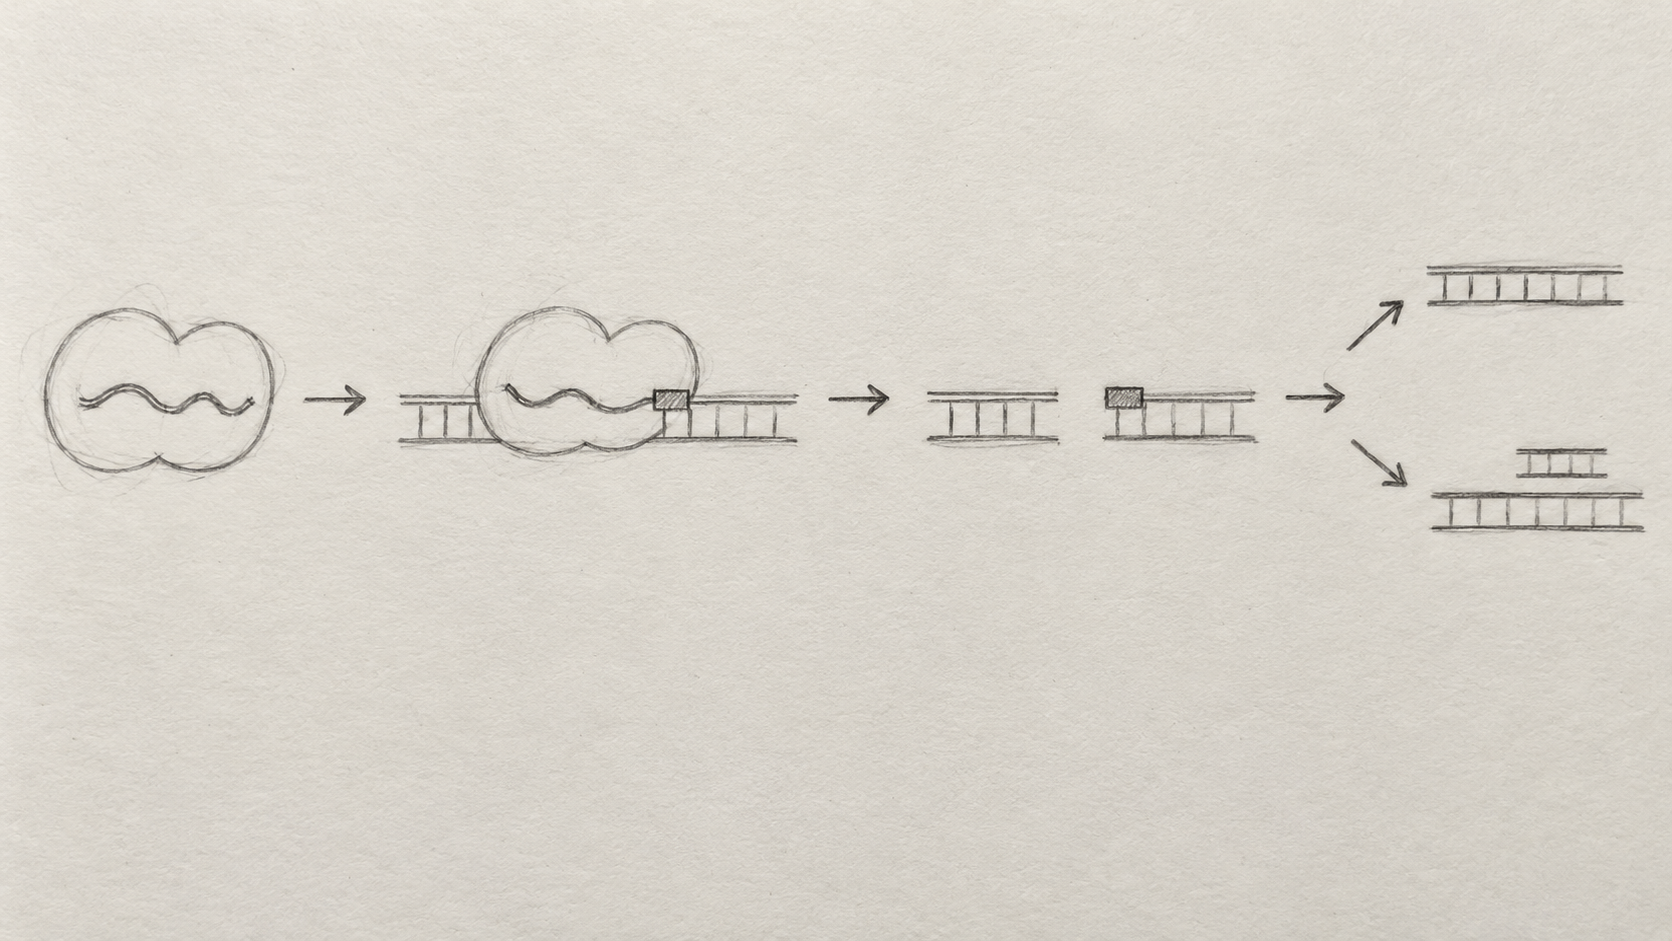
\includegraphics[width=\linewidth]{figures/ch03/ch03-02a-sketch-linear.png}};
\begin{scope}[x={(img.south east)},y={(img.north west)}]
  \node[font=\sffamily\bfseries\normalsize, anchor=north west, text=BookInk] at (0.04,0.94) {A};
\end{scope}
\end{tikzpicture}\\[1mm]
{\footnotesize A\quad Linear (left $\rightarrow$ right)}
\end{minipage}\hfill
\begin{minipage}[t]{0.32\linewidth}\centering
\begin{tikzpicture}
\node[anchor=south west,inner sep=0] (img) at (0,0) {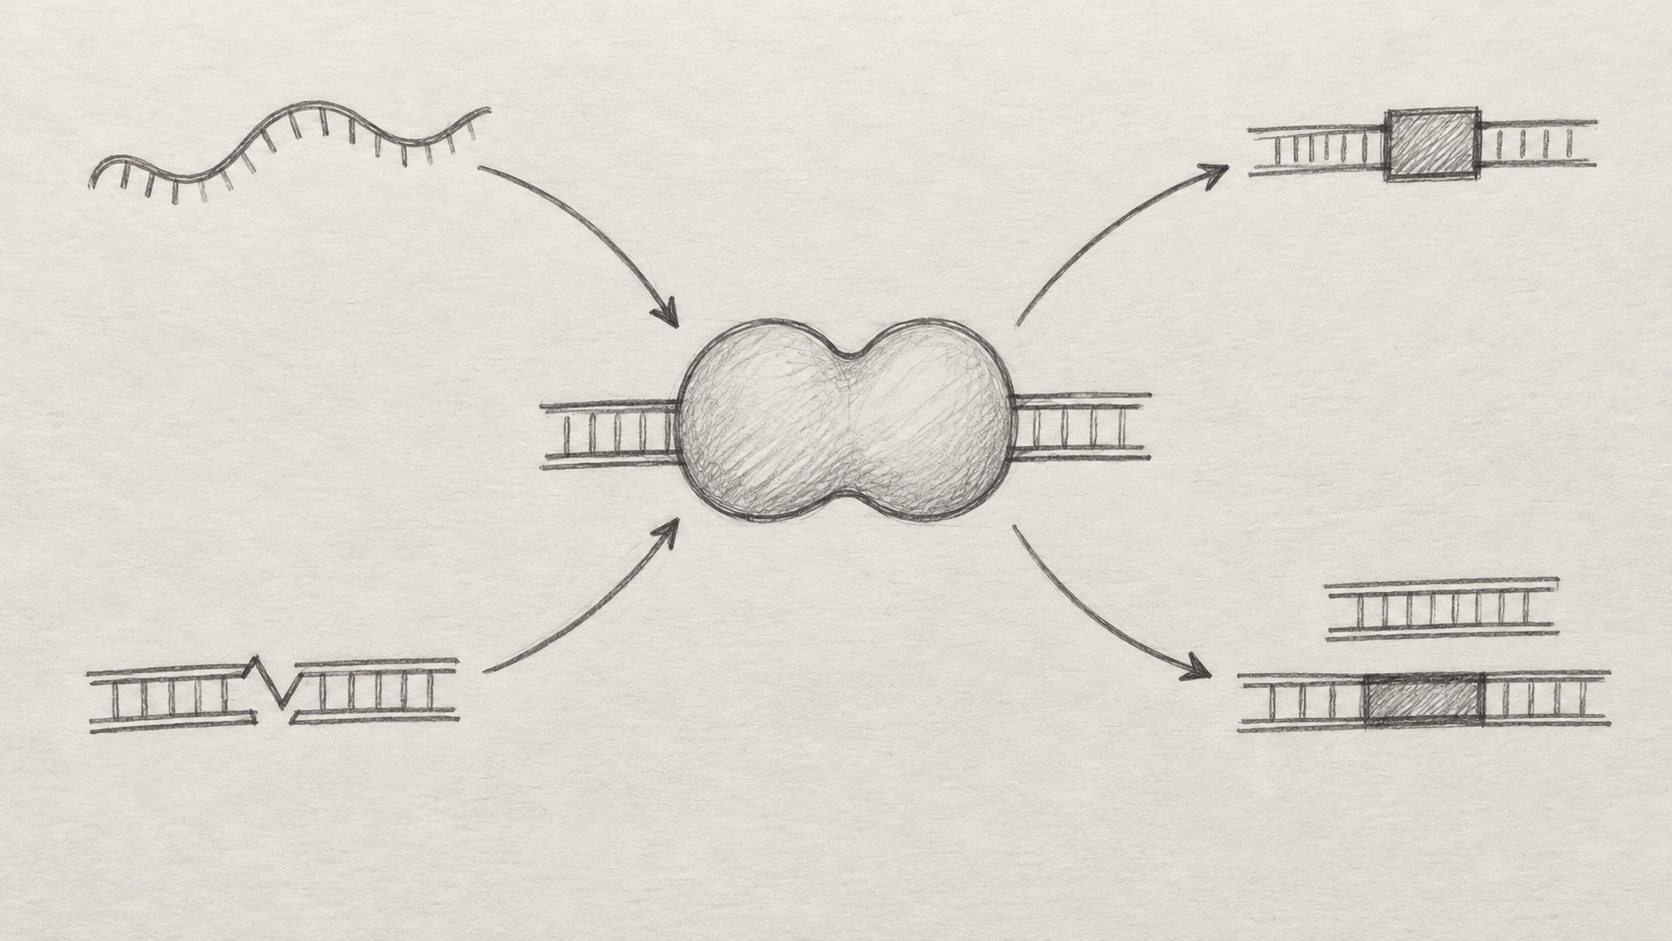
\includegraphics[width=\linewidth]{figures/ch03/ch03-02b-sketch-hub.png}};
\begin{scope}[x={(img.south east)},y={(img.north west)}]
  \node[font=\sffamily\bfseries\normalsize, anchor=north west, text=BookInk] at (0.04,0.94) {B};
\end{scope}
\end{tikzpicture}\\[1mm]
{\footnotesize B\quad Hub}
\end{minipage}\hfill
\begin{minipage}[t]{0.32\linewidth}\centering
\begin{tikzpicture}
\node[anchor=south west,inner sep=0] (img) at (0,0) {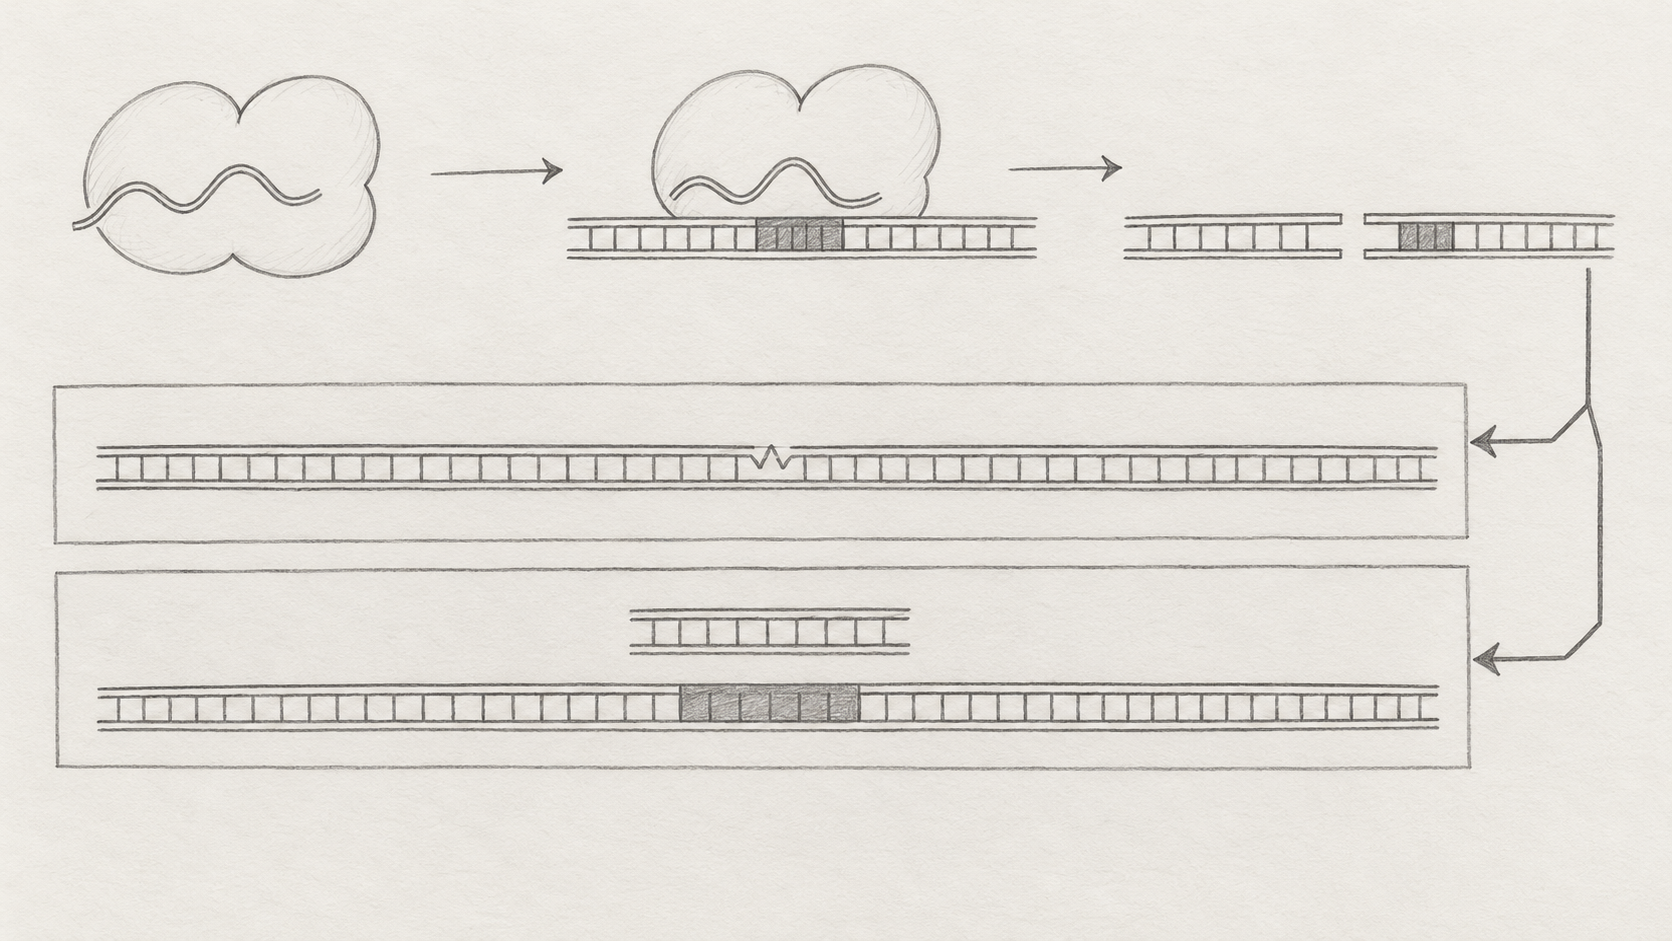
\includegraphics[width=\linewidth]{figures/ch03/ch03-02c-sketch-branch.png}};
\begin{scope}[x={(img.south east)},y={(img.north west)}]
  \node[font=\sffamily\bfseries\normalsize, anchor=north west, text=BookInk] at (0.04,0.94) {C};
\end{scope}
\end{tikzpicture}\\[1mm]
{\footnotesize C\quad Two-branch outcome}
\end{minipage}
\caption{Three layout skeletons for the same content (pencil sketches simulated with an image model). A sketch fixes regions, relative sizes, arrow directions, and white space, and carries no text; what each shape means is defined in the brief. A arranges the events in a single row, B centers on the Cas9--DNA complex, and C compresses the first three steps into a top row above two parallel repair lanes. The example figures in this chapter were generated with an image model; prompts and generation records are available in the book repository.}\label{fig:ch03-02}
\end{figure}

Inspecting the actual images and generation history of Figure~\ref{fig:ch03-02} yields three practical observations:

First, \textbf{a single-row linear layout succeeds on the first try, but squeezes the right-hand comparison region.} Figure~\ref{fig:ch03-02}A formed the four left-to-right stages and right-hand fork on the first sample, but because the first three steps take up most of the width, the two stacked outcome duplexes on the far right are compressed into very short segments.

Second, \textbf{a central hub layout inherently erases a unique entry point.} When generating Figure~\ref{fig:ch03-02}B, the first sample drew the bottom-left indel zigzag as a detached lightning bolt and pointed arrows inward from the right corners. The second sample restored the small zigzag attached to the DNA duplex, with single-headed arrows pointing inward from top-left and bottom-left and outward to top-right and bottom-right (with heavier pencil shading on the central protein), leaving no single entry point.

Third, \textbf{image models struggle with branched arrow routing into separate containers.} When generating Figure~\ref{fig:ch03-02}C, the first two samples drew the top row and the two lower pencil frames, but both times pointed \textbf{both branches of the split arrow onto the top edge of the upper frame}, leaving the lower lane without an entry arrow and splitting the upper DNA into a wide gap. Only on the third sample—after adding explicit routing instructions so the trunk runs down the right margin, sending one branch into the right end of the upper frame and the other into the right end of the lower frame, while keeping the upper DNA continuous around a small central zigzag—did the model connect both lanes properly. Even in Figure~\ref{fig:ch03-02}C, the two pencil boxes differ slightly in height (the lower box is taller) and the RNA inside the top-left protein has a double line. Sketching boxes and a split arrow by hand with a pencil takes a minute and avoids guessing topology through text.

Before moving on, check each sketch against four points: clear entry point, unambiguous fork into parallel outcomes, enough whitespace for labels, and zero text.

\section{From Sketches to Candidates, Then a Choice}

Next, we switch to \textbf{Sketch Mode} in the \scidraw{} prompt drawing tool (\sdtool{ai-drawing}), upload each sketch in turn, and paste the same English prompt derived from our brief. Changing only the uploaded sketch and the final layout line keeps visual style, color identities, step definitions, and exclusions identical for a fair test:

\begin{Prompt}
Flat 2D scientific overview schematic for a journal figure, landscape 16:9, pure white background. Clean vector illustration style: flat fills, thin dark gray outlines, no gradients, no shadows, no highlights, no 3D, no glow, no texture. ABSOLUTELY NO TEXT: no letters, no words, no numbers, no symbols, no labels, no legend, no title.
Follow the layout of the attached pencil sketch closely: same regions, same relative positions, same arrow directions.
OBJECTS (use these exact visual identities in every step where they appear):
- Cas9: a rounded two-lobed protein shape, muted blue-gray (#7C93A8).
- sgRNA: a single orange (#E69F00) strand with a short straight segment (the spacer) and a small hairpin loop scaffold, partly inside Cas9.
- Genomic DNA: two parallel dark gray (#4D4D4D) lines with short light gray rungs between them.
- PAM: a short bright yellow (#F0E442) segment on the upper DNA line.
- Double-strand break: a clean gap through both DNA lines, right next to the PAM.
- Donor template: a short separate double-stranded DNA; its two ends dark gray (homology arms), its middle segment teal (#009E73).
- NHEJ result: a continuous DNA with one small reddish-purple (#CC79A7) mark at the former break site.
- HDR result: a continuous DNA with a teal (#009E73) segment at the former break site, the same length as the donor's middle segment.
\end{Prompt}

\begin{Prompt}
STEPS: (1) Cas9 bound to sgRNA. (2) Cas9-sgRNA sitting on the DNA at the PAM, the orange spacer lying alongside the lower DNA line, the upper line slightly pushed away. (3) The DNA with the break next to the PAM, Cas9 lifted away. (4) Repair by end joining, giving the NHEJ result, with no donor. (5) Repair using the donor template, giving the HDR result; the donor appears only here. Steps are connected by solid dark gray arrows with filled heads; after step 3 the arrow splits into two equal arrows.
DO NOT DRAW: cells, nucleus, chromosomes, scissors, lightning, sparkles, double-helix twisting, realistic protein structure, any charts or data. Bottom 10% of the image empty.
LAYOUT [A]: one row of five steps left to right; steps 4 and 5 stacked at the right end.
LAYOUT [B]: radial; the DNA-bound Cas9 complex (step 2-3 merged) in the center, steps 1, 4, 5 and the PAM detail around it.
LAYOUT [C]: steps 1-3 as a compact row across the top third; below, two equal-height horizontal lanes stacked vertically, upper lane step 4, lower lane step 5, with the DNA in both lanes aligned at the same x positions and length.
\end{Prompt}

Keep one boundary in mind: \textbf{a sketch is a strong layout hint, not a pixel-level layout lock.} When rendering pencil lines into colored shapes, the model can still shift positions, duplicate markers, or swap object identities. After generation, we check each candidate against its sketch and overlay orange reading-order numbers (Figure~\ref{fig:ch03-03}).

\begin{figure}[htbp]\centering
\begin{minipage}[t]{0.32\linewidth}\centering
\begin{tikzpicture}[ord/.style={circle, draw=orange!85!black, line width=0.6pt, fill=orange!15, inner sep=1pt, font=\sffamily\bfseries\scriptsize, text=BookInk}]
\node[anchor=south west,inner sep=0] (img) at (0,0) {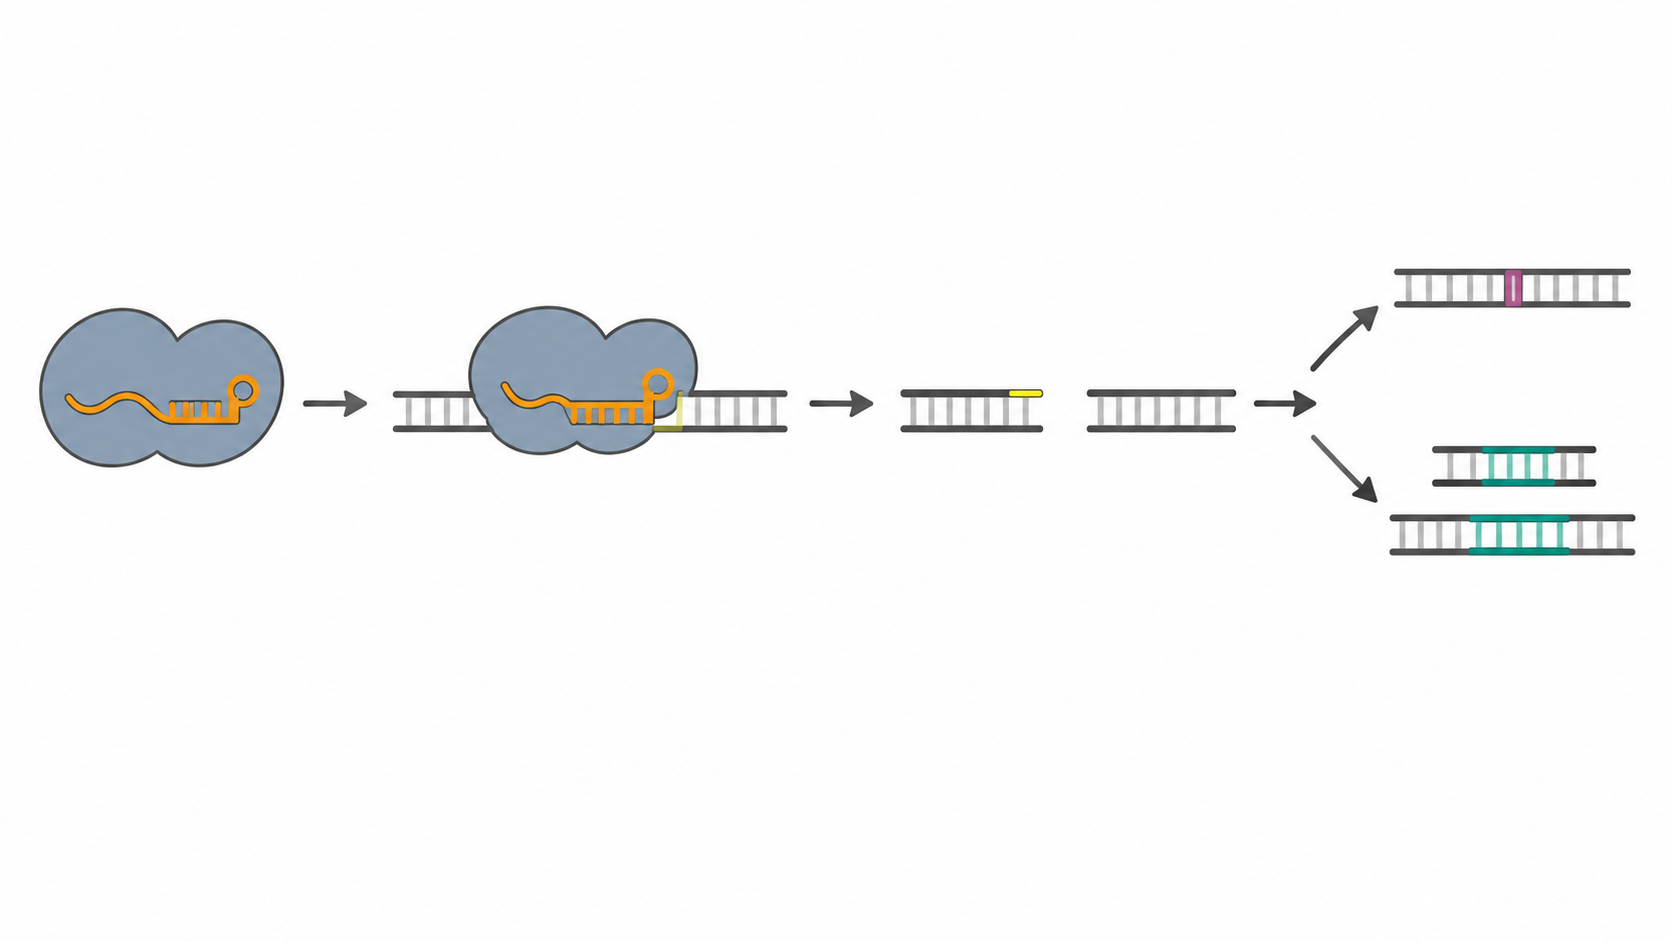
\includegraphics[width=\linewidth]{figures/ch03/ch03-03a-cand-linear.png}};
\begin{scope}[x={(img.south east)},y={(img.north west)}]
  \node[font=\sffamily\bfseries\normalsize, anchor=north west, text=BookInk] at (0.04,0.94) {A};
  \node[ord] at (0.08,0.55) {1};
  \node[ord] at (0.27,0.55) {2};
  \node[ord] at (0.46,0.55) {3};
  \node[ord] at (0.80,0.72) {4};
  \node[ord] at (0.80,0.35) {5};
\end{scope}
\end{tikzpicture}
\end{minipage}\hfill
\begin{minipage}[t]{0.32\linewidth}\centering
\begin{tikzpicture}[ord/.style={circle, draw=orange!85!black, line width=0.6pt, fill=orange!15, inner sep=1pt, font=\sffamily\bfseries\scriptsize, text=BookInk}]
\node[anchor=south west,inner sep=0] (img) at (0,0) {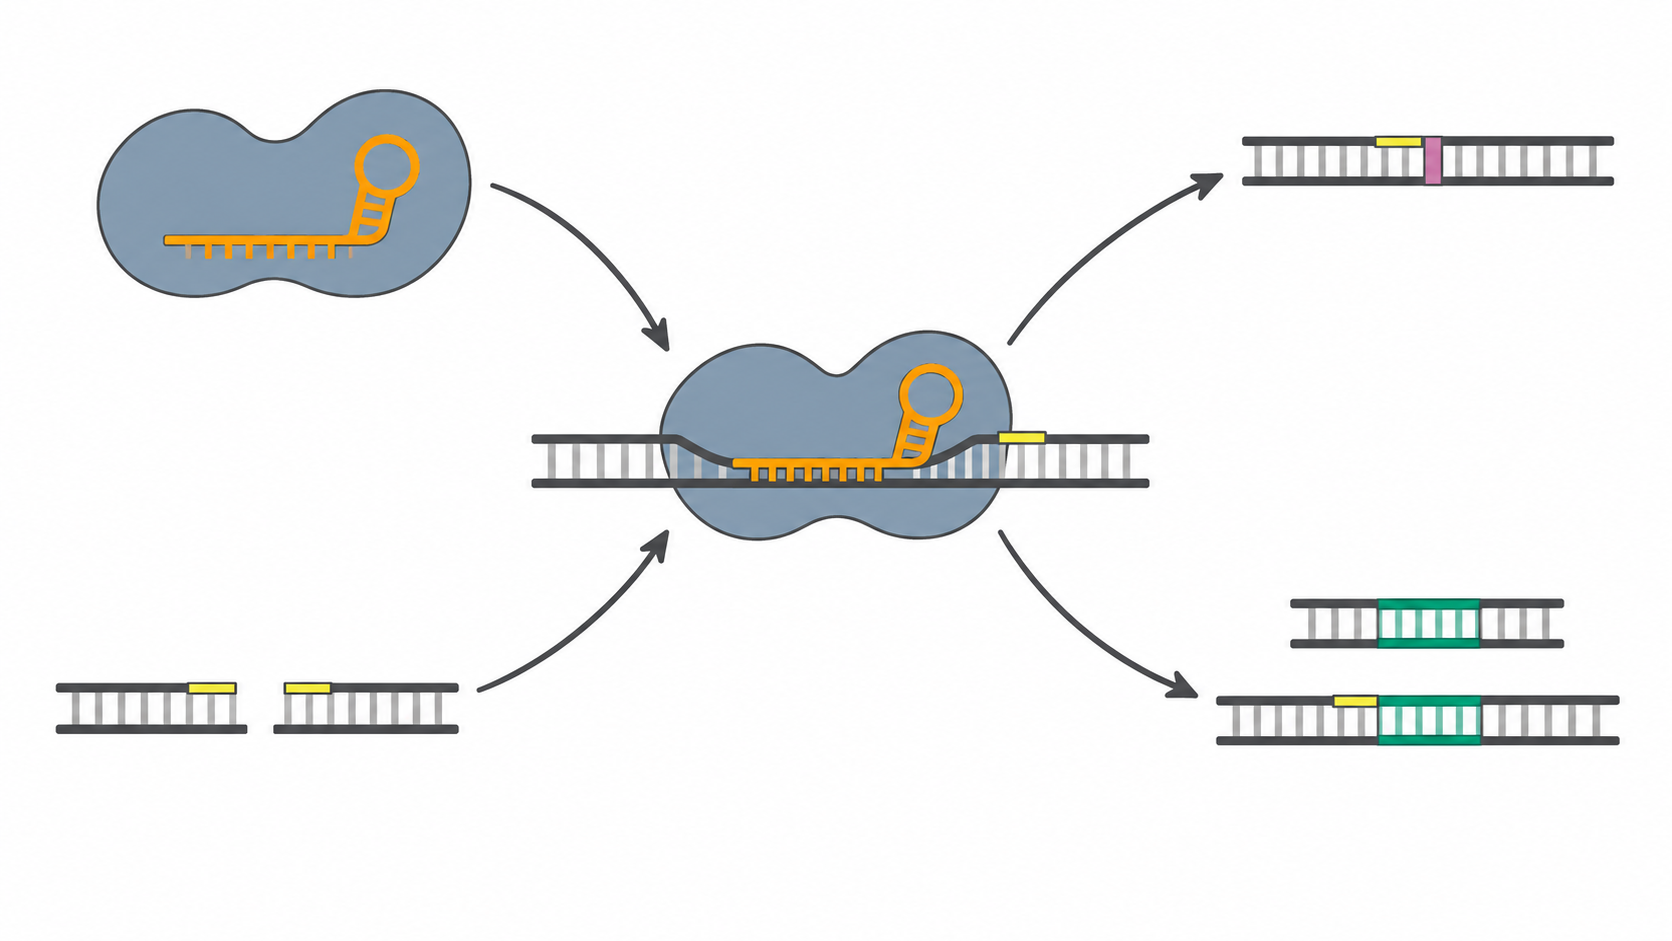
\includegraphics[width=\linewidth]{figures/ch03/ch03-03b-cand-hub.png}};
\begin{scope}[x={(img.south east)},y={(img.north west)}]
  \node[font=\sffamily\bfseries\normalsize, anchor=north west, text=BookInk] at (0.04,0.94) {B};
  \node[ord] at (0.50,0.52) {1?};
\end{scope}
\end{tikzpicture}
\end{minipage}\hfill
\begin{minipage}[t]{0.32\linewidth}\centering
\begin{tikzpicture}[ord/.style={circle, draw=orange!85!black, line width=0.6pt, fill=orange!15, inner sep=1pt, font=\sffamily\bfseries\scriptsize, text=BookInk}]
\node[anchor=south west,inner sep=0] (img) at (0,0) {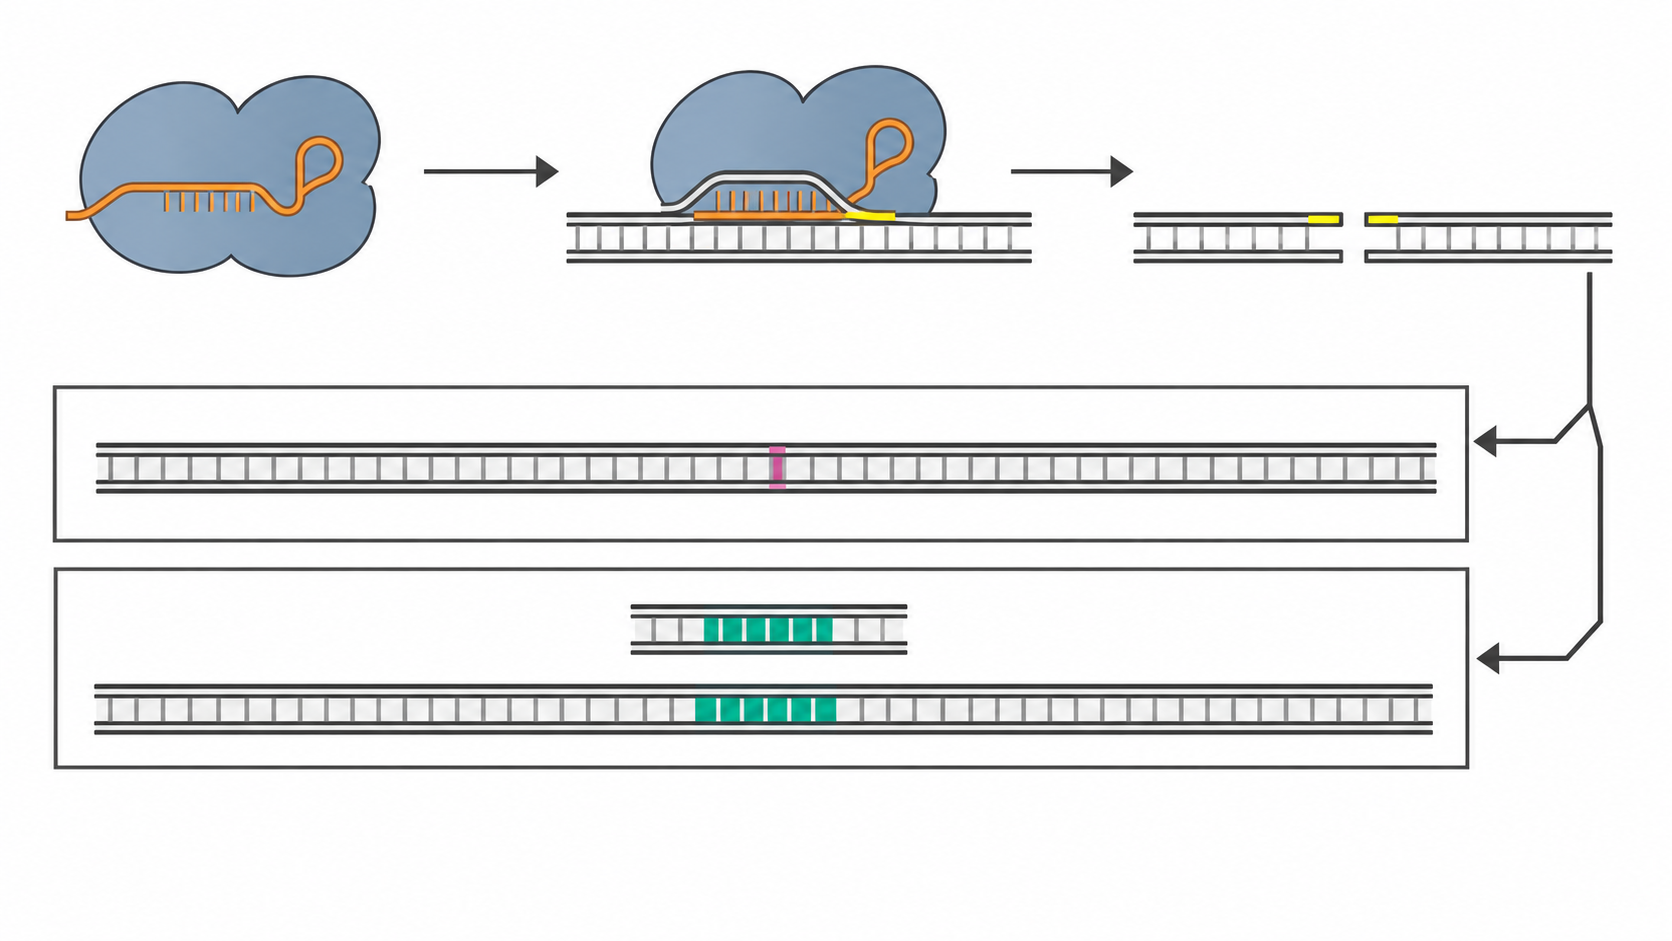
\includegraphics[width=\linewidth]{figures/ch03/ch03-03c-cand-branch.png}};
\begin{scope}[x={(img.south east)},y={(img.north west)}]
  \node[font=\sffamily\bfseries\normalsize, anchor=north west, text=BookInk] at (0.04,0.94) {C};
  \node[ord] at (0.15,0.85) {1};
  \node[ord] at (0.38,0.85) {2};
  \node[ord] at (0.62,0.85) {3};
  \node[ord] at (0.50,0.55) {4};
  \node[ord] at (0.50,0.22) {5};
\end{scope}
\end{tikzpicture}
\end{minipage}
\caption{Candidates generated from one brief and three different sketches. Orange numbers indicate the author's intended reading order (in an active project, test unnumbered prints with colleagues who have not seen the brief): in A and C the order is clear and matches the sequence of events; in B both top-left and bottom-left arrows point inward toward the center, leaving no unique entry point. Each candidate was checked against its input sketch for positional drift.}\label{fig:ch03-03}
\end{figure}

Comparing Figure~\ref{fig:ch03-02} and Figure~\ref{fig:ch03-03} side by side shows how each skeleton performed and where positional drift occurred:

\begin{itemize}
\item \textbf{Candidate A (Linear, Figure~\ref{fig:ch03-03}A):} Succeeded on the first sample in following Sketch A's single row, with accurate colors for Cas9 (blue-gray), sgRNA (orange), DNA (dark gray), PAM (yellow), indel (reddish-purple), and donor/insert (teal), placing the donor only at bottom right. However, Step 3 (cleavage) shows a classic \textbf{positional drift}: the PAM block on the \textbf{right} of the gap in Sketch A shifted to the \textbf{left} of the gap in Candidate A; R-loop pairing in Step 2 is also indistinct, the stacked outcomes on the right are cramped, and the donor's teal segment differs slightly in length from the HDR insert.
\item \textbf{Candidate B (Hub, Figure~\ref{fig:ch03-03}B):} Vividly shows how a flawed layout skeleton induces scientific errors. The first two samples reversed the bottom-left arrow outward (turning top-left into a pseudo-entry and expanding the lone sgRNA into a Cas9--sgRNA complex) or drew a double-headed arrow. After the third sample enforced two inward arrows from the left and two outward arrows to the right, arrow directions matched the sketch, but severe \textbf{identity swapping and marker proliferation} occurred: the NHEJ outcome (reddish-purple mark) moved from bottom-left to top-right while bottom-left became cleaved DNA; extra yellow PAM blocks appeared on both sides of the bottom-left gap, left of the top-right reddish-purple mark, and left of the bottom-right teal insert, while the central complex shows no clear break. Treating ``sgRNA,'' ``cleaved DNA,'' and ``repair outcomes'' as equal satellites also flattens the event hierarchy.
\item \textbf{Candidate C (Two-branch, Figure~\ref{fig:ch03-03}C):} Retained the ``compact three-step top row + right fork + stacked parallel lanes'' on the first sample; the short donor appears only in the lower HDR lane centered above the teal insert, the two long DNA strands align horizontally within 0.3\% of strand length, and no forbidden objects appear. Zooming in reveals two defects to fix: first, at Step 3 in the top row, \textbf{yellow PAM blocks appear on both the left and right sides of the gap} (duplicate PAM); second, the two rectangular lane frames differ in height, with the lower frame about 29\% taller than the upper frame (and all three candidates show slight shading/highlights on proteins and orange strands rather than purely flat fills).
\end{itemize}

In practice, show the unnumbered candidates to one or two colleagues who have not seen the brief and ask them to number steps 1--5 (a vision-capable conversational AI can offer a secondary check, but cannot replace human readers). Then evaluate the candidates with a criteria table (Table~\ref{tab:ch03-02-cmp} and Figure~\ref{fig:ch03-04}) rather than gut preference.

\begin{table}[htbp]\centering\footnotesize
\setlength{\tabcolsep}{3pt}
\renewcommand{\arraystretch}{1.15}
\caption{Comparison of the three candidate layout structures.}\label{tab:ch03-02-cmp}
\begin{tabularx}{\linewidth}{@{}>{\raggedright\arraybackslash}p{36mm}YYY@{}}
\toprule
\textbf{Criterion} & \textbf{A: Linear} & \textbf{B: Central Hub} & \textbf{C: Two-Branch} \\
\midrule
Single, unambiguous entry point & Yes (left Step 1) & No (two inward arrows from left corners) & Yes (top-left Step 1) \\
Reading direction matches event order & Yes & Partial (relies on arrows; objects swapped) & Yes \\
Outcomes directly comparable on shared baseline & No (stacked tightly at right end) & No (split between top-right and bottom-right) & Yes (stacked wide lanes, aligned endpoints) \\
Visual weight of main message (one break, two outcomes) & Low ($\approx$11\%--25\% at right) & Medium ($\approx$25\% in corners) & High ($\approx$50\% across lower half) \\
Label space at 174 mm width & Tight & Moderate & Generous \\
Best suited for & Stepwise slide animation & Non-sequential concept map & Journal overview figure \\
\bottomrule
\end{tabularx}
\end{table}

\begin{figure}[htbp]\centering
\resizebox{\linewidth}{!}{% FIG ch03-04 layout comparison (English)
\begin{tikzpicture}[
  x=1mm, y=1mm,
  font=\sffamily\footnotesize,
  text=BookInk,
  wf/.style={draw=black!50, fill=black!4, line width=0.4pt},
  main/.style={fill=teal!25, draw=none},
]
  \def\fw{52}\def\fh{33}
  \begin{scope}[shift={(0,58)}]
    \draw[wf] (0,0) rectangle (\fw,\fh);
    \fill[main] (0.68*\fw,0.05*\fh) rectangle (0.96*\fw,0.43*\fh);
    \node[anchor=north, font=\bfseries] at (0.5*\fw,\fh+2) {A};
    \node[font=\scriptsize, anchor=south] at (0.5*\fw,-1.5) {$\approx$11\%};
  \end{scope}
  \begin{scope}[shift={(56,58)}]
    \draw[wf] (0,0) rectangle (\fw,\fh);
    \fill[main] (0.15*\fw,0.12*\fh) rectangle (0.85*\fw,0.47*\fh);
    \node[anchor=north, font=\bfseries] at (0.5*\fw,\fh+2) {B};
    \node[font=\scriptsize, anchor=south] at (0.5*\fw,-1.5) {$\approx$25\%};
  \end{scope}
  \begin{scope}[shift={(112,58)}]
    \draw[wf] (0,0) rectangle (\fw,\fh);
    \fill[main] (0,0) rectangle (\fw,0.50*\fh);
    \node[anchor=north, font=\bfseries] at (0.5*\fw,\fh+2) {C};
    \node[font=\scriptsize, anchor=south] at (0.5*\fw,-1.5) {$\approx$50\%};
  \end{scope}
  \node[font=\scriptsize, text=BookInk!70, anchor=north west] at (0,54)
    {Teal: area for the two repair outcomes (wireframe proxy; update after PNG measurement).};

  \matrix (m) [
    matrix of nodes,
    anchor=north west,
    row sep=1.8mm,
    column sep=3mm,
    nodes={font=\scriptsize, inner sep=2pt},
    column 1/.style={nodes={anchor=west}, text width=42mm},
    column 2/.style={nodes={anchor=center}, text width=12mm},
    column 3/.style={nodes={anchor=center}, text width=12mm},
    column 4/.style={nodes={anchor=center}, text width=12mm},
  ] at (0,48) {
    & {A} & {B} & {C} \\
    Single entry point & {$\bullet$} & {$\circ$} & {$\bullet$} \\
    Order matches events & {$\bullet$} & {\tikz[baseline=-0.6ex]{\fill[BookTeal] (0,0) arc (90:270:0.35); \draw[BookTeal] (0,0) circle (0.35);}} & {$\bullet$} \\
    Outcomes directly comparable & {$\circ$} & {$\circ$} & {$\bullet$} \\
    Area for main message & {$\circ$} & {\tikz[baseline=-0.6ex]{\fill[BookTeal] (0,0) arc (90:270:0.35); \draw[BookTeal] (0,0) circle (0.35);}} & {$\bullet$} \\
    Label space at 174\,mm & {\tikz[baseline=-0.6ex]{\fill[BookTeal] (0,0) arc (90:270:0.35); \draw[BookTeal] (0,0) circle (0.35);}} & {\tikz[baseline=-0.6ex]{\fill[BookTeal] (0,0) arc (90:270:0.35); \draw[BookTeal] (0,0) circle (0.35);}} & {$\bullet$} \\
    Best suited for & {Slides} & {Concept map} & {Paper overview} \\
  };
  \draw[BookTeal, line width=0.8pt, rounded corners=1pt]
    ([xshift=-2mm,yshift=2mm]m-1-4.north west) rectangle ([xshift=2mm,yshift=-2mm]m-7-4.south east);
\end{tikzpicture}
}
\caption{Comparing the three layouts against stated criteria. Top: in each wireframe, the teal area represents the proportion of layout space given to the two repair outcomes. Bottom: criterion-by-criterion assessment matrix. Layout C was chosen for the paper overview; A was kept for a stepwise slide version.}\label{fig:ch03-04}
\end{figure}

As Figure~\ref{fig:ch03-04} shows, because the core message is ``one break, two repair outcomes,'' Layout C devotes roughly 50\% of the canvas to the two aligned repair lanes so readers can directly compare the indel and precise edit at the same horizontal position. We record our rationale: \textbf{select C for the paper overview figure; retain A for stepwise presentation slides; discard B.}

\section{One Verifiable Goal per Revision}

When revising Candidate C, avoid bundled prompts such as ``fix the details, align the lanes, and make it cleaner.'' Reference-image editing in \scidraw{} (selecting a history image and entering an edit prompt) is conditional resampling, not vector translation; bundling multiple goals makes it impossible to tell which clause caused an unintended change.

Follow a strict revision discipline: \textbf{state only one verifiable goal per pass using ``target change + what stays unchanged + verification check,'' compare each output against the previous version by overlay, and log all unrequested changes.}

We first diagnose four checkpoints (1 to 4) on Candidate C (Figure~\ref{fig:ch03-05}, left):

\begin{itemize}
\item \textbf{Checkpoint 1 (PAM position):} Step 3 in the top row has yellow PAM blocks on both sides of the cleavage gap; we must \textbf{remove the left yellow block and keep only the upper-strand PAM immediately to the right of the gap}.
\item \textbf{Checkpoint 2 (Donor placement):} Although we worried the donor might float between lanes or duplicate, in Candidate C it already sits uniquely inside the lower HDR lane roughly centered over the edit. To test single-goal fine-tuning and center its teal middle segment strictly above the inserted segment, we still run one micro-adjustment pass.
\item \textbf{Checkpoint 3 (Lane alignment):} The two long DNA duplexes already align horizontally within 0.3\% ($<2\%$ target), but \textbf{the two rectangular lane frames differ in height by about 29\%} (lower frame taller than upper frame) and need equalizing.
\item \textbf{Checkpoint 4 (Extra background objects):} Prepared conditionally in case a cell nucleus or background shape appeared; Candidate C has a clean background, so \textbf{Revision 4 is skipped}.
\end{itemize}

The four single-goal revision prompts are:

\begin{Prompt}
[Revision 1 - PAM position] Edit the selected image. Change only one thing: move the small yellow PAM segment so that it sits directly next to the right side of the DNA gap at the cleavage step, on the upper strand, touching the gap. Keep every other object, color, line weight and position unchanged. Do not add any text.
\end{Prompt}

\begin{Prompt}
[Revision 2 - Donor placement] Edit the selected image. Change only one thing: move the short teal donor DNA so that it lies inside the lower repair lane only, directly above the DNA gap in that lane, horizontally centered on the gap. Remove any copy of the donor outside the lower lane. Keep everything else unchanged. No text.
\end{Prompt}

\begin{Prompt}
[Revision 3 - Lane alignment] Edit the selected image. Change only one thing: make the two repair lanes the same height, and draw the DNA in both lanes at the same horizontal position and the same length, so the two results line up vertically for comparison. Keep colors, objects and the top row unchanged. No text.
\end{Prompt}

\begin{Prompt}
[Revision 4 - Remove extra objects, conditional] Edit the selected image. Remove the cell nucleus outline and any background shapes. Change nothing else. No text.
\end{Prompt}

\begin{figure}[htbp]\centering
\begin{minipage}[t]{0.49\linewidth}\centering
\begin{tikzpicture}[font=\sffamily\footnotesize, text=BookInk]
  \node[inner sep=0, anchor=south west] (imga) at (0,0) {%
    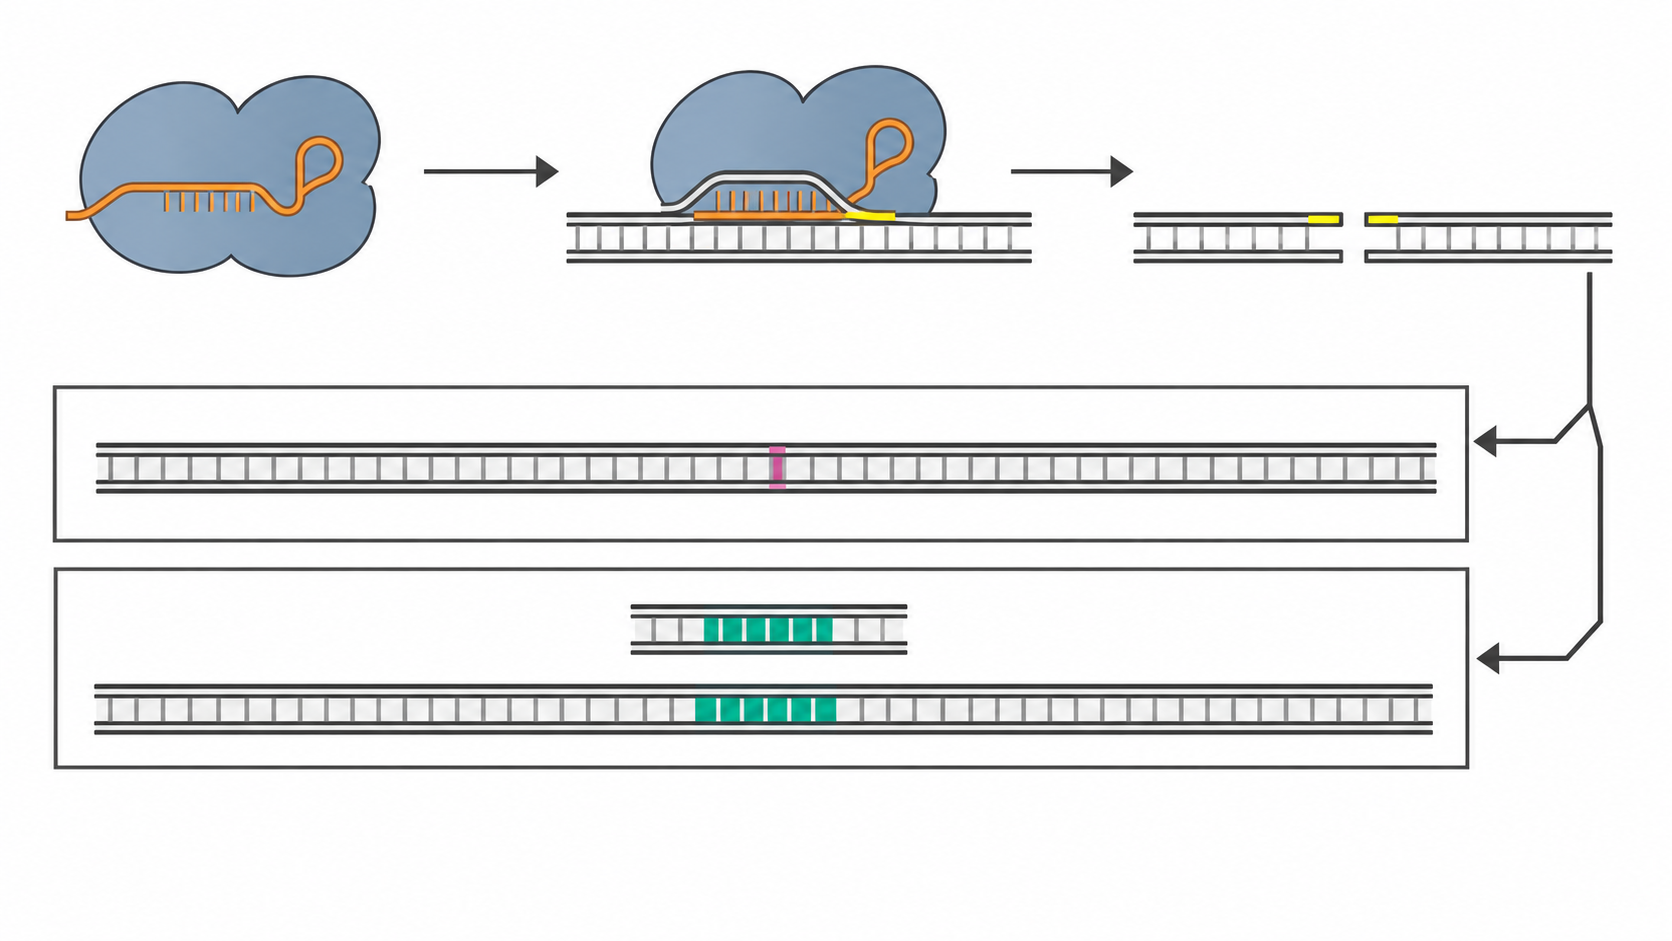
\includegraphics[width=\linewidth]{figures/ch03/ch03-03c-cand-branch.png}};
  \begin{scope}[x={(imga.south east)},y={(imga.north west)},
    issuemark/.style={circle, draw=red!75!black, line width=0.6pt, fill=white, fill opacity=0.88, text opacity=1, inner sep=0.8pt, font=\sffamily\bfseries\scriptsize, text=red!75!black}]
    \node[issuemark] at (0.62,0.78) {1};
    \node[issuemark] at (0.48,0.42) {2};
    \node[issuemark] at (0.72,0.28) {3};
    \node[issuemark] at (0.88,0.65) {4};
    \node[anchor=west, align=left, font=\sffamily\scriptsize] at (0.02,0.08) {%
      1 PAM position\quad 2 Donor placement\\
      3 Lanes misaligned\quad 4 Extra-object check};
  \end{scope}
\end{tikzpicture}
\end{minipage}\hfill
\begin{minipage}[t]{0.49\linewidth}\centering
\begin{tikzpicture}[font=\sffamily\footnotesize, text=BookInk]
  \node[inner sep=0, anchor=south west] (imgb) at (0,0) {%
    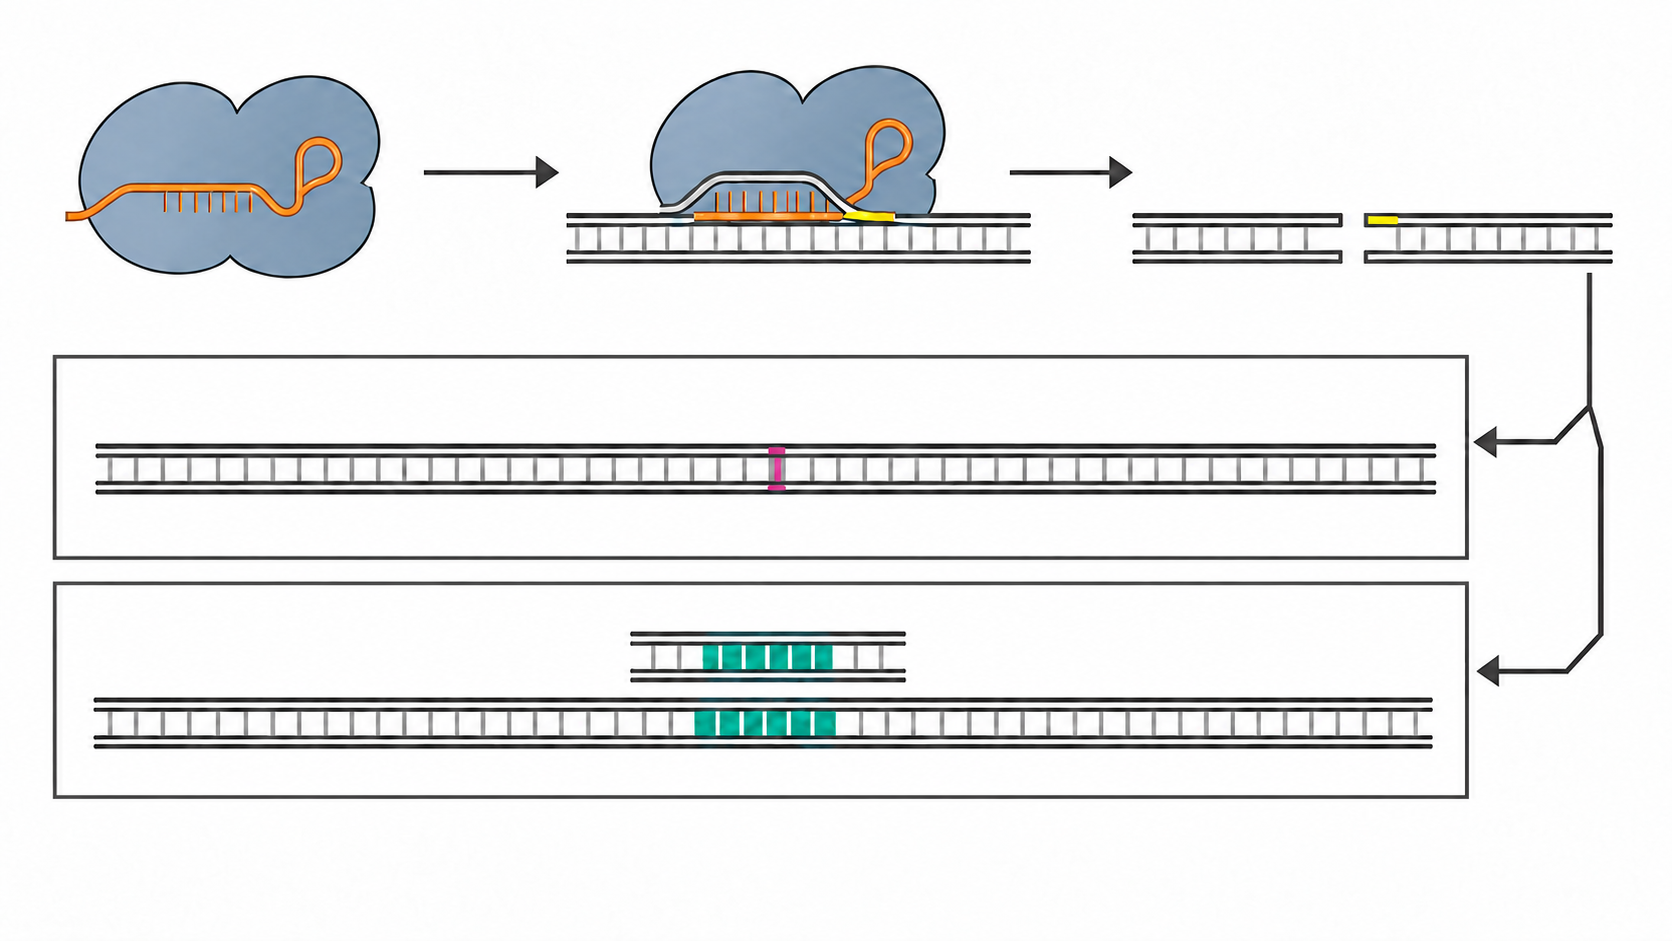
\includegraphics[width=\linewidth]{figures/ch03/ch03-05b-v3-revised.png}};
  \begin{scope}[x={(imgb.south east)},y={(imgb.north west)}]
    \draw[green!55!black, line width=0.8pt] (0.14,0.80) circle (0.07);
    \draw[green!55!black, line width=0.8pt] (0.48,0.29) circle (0.09);
    \node[anchor=west, align=left, font=\sffamily\tiny, text=green!45!black] at (0.02,0.08) {%
      Unrequested: sgRNA highlight redrawn,\\
      lower lane shifted \& $\sim$6\% frame gap};
  \end{scope}
\end{tikzpicture}
\end{minipage}
\caption{One change at a time. Left: four diagnostic checkpoints on Candidate C, where checkpoint 1 has duplicate yellow PAM blocks on both sides of the cleavage gap and checkpoint 3 has unequal lane frame heights (checkpoint 2 already has the donor inside the lower lane, and checkpoint 4 confirms no extra background objects). Right: the version after sequential single-goal edits; the duplicate left PAM is removed and the frame-height discrepancy is greatly reduced. Green circles mark minor unrequested redrawing and vertical shift recorded in the revision log.}\label{fig:ch03-05}
\end{figure}

Table~\ref{tab:ch03-03-log} records the seven actual edit calls from Candidate C to Figure~\ref{fig:ch03-05} (right) and how unrequested changes were handled:

\begin{table}[htbp]\centering\footnotesize
\setlength{\tabcolsep}{3pt}
\renewcommand{\arraystretch}{1.15}
\caption{Unrequested-change log from Candidate C to the revised draft.}\label{tab:ch03-03-log}
\begin{tabularx}{\linewidth}{@{}>{\raggedright\arraybackslash}p{25mm}ccY>{\raggedright\arraybackslash}p{22mm}@{}}
\toprule
\textbf{Revision Stage} & \textbf{Try} & \textbf{Goal Met?} & \textbf{Unrequested Changes (and Scientific Impact)} & \textbf{Decision} \\
\midrule
Rev 1: PAM position & 1 & No & Duplicate yellow PAM blocks remain on both sides of gap; minor line re-rendering (no scientific impact) & Revert to Candidate C \\
Rev 1: Explicit locus & 2 & \textbf{Yes} & Left duplicate PAM removed; subtle outline and texture re-rendering (no impact) & \textbf{Keep} as Baseline 1 \\
Rev 2: Donor centering & 1 & No & \textbf{Sole short donor duplex in lower lane deleted entirely (breaks scientific content)} & \textbf{Discard}; revert to Baseline 1 \\
Rev 2: Protect donor & 2 & \textbf{Yes} & Donor retained and centered over teal insert; donor shifted slightly downward (no impact) & \textbf{Keep} as Baseline 2 \\
Rev 3: Equal lane height & 1 & Partial & \textbf{Donor vanished; both outcome DNAs acquired both reddish-purple and teal marks (breaks science)} & \textbf{Discard}; revert to Baseline 2 \\
Rev 3: Protect identities & 2 & No & Scientific identities restored, but lower frame stretched taller and shifted down (geometry failed) & Discard; revert to Baseline 2 \\
Rev 3: Raise upper frame & 3 & \textbf{Yes} & Frame-height gap reduced from 29.4\% to 6.0\%, endpoint error 0.22\%; slight lower-lane shift and sgRNA highlight change (no impact) & \textbf{Keep} as Revised Draft \\
Rev 4: Remove background & 0 & --- & No cell nucleus or extraneous background shapes present & Conditionally skipped \\
\bottomrule
\end{tabularx}
\end{table}

Three practical rules emerge from Table~\ref{tab:ch03-03-log}:

\textbf{First, when an initial instruction fails, add explicit localization stating what is wrong, what to erase, and what to keep.} Try 1 of Revision 1 failed because a yellow PAM block already sat to the right of the gap, so the model left the extra left yellow block intact; specifying on Try 2 to ``erase the left yellow highlight back to dark-gray DNA and keep only the upper-strand yellow segment right of the gap'' worked immediately.

\textbf{Second, watch for destructive side effects—deleting a unique object or homogenizing contrasting outcomes—and revert immediately to the previous verified baseline.} On Try 1 of Revision 2, over-responding to ``Remove any copy'' erased the only donor template; on Try 1 of Revision 3, over-responding to ``same height and length'' deleted the donor and painted \emph{both} outcome duplexes with both reddish-purple and teal marks, destroying the NHEJ versus HDR comparison! Never patch a scientifically broken output; \textbf{step straight back to the previous verified baseline} and add protective constraints (e.g., keeping only the reddish-purple mark in the upper lane, keeping the teal insert and donor in the lower lane, and raising only the top edge of the upper frame).

\textbf{Third, separate scientific errors from harmless rendering drift, and switch to deterministic tools when needed.} The green circles in Figure~\ref{fig:ch03-05} (right) mark minor cumulative drift: slight changes in sgRNA highlight and stroke weight, a tiny downward shift of the lower lane, and a residual 6.0\% frame-height difference (down from 29.4\%, with DNA endpoints aligned within 0.22\%). Because these do not affect C1--C9, we log them and accept the draft. If a local edit still breaks key objects after three tries, stop resampling and draw exact geometry in TikZ.

\section{Closing the Case: Final Figure, Legend, and Verification}

To reserve space in the upper-right corner for the deterministic PAM inset (Figure~\ref{fig:ch03-07}), we run one final whitespace edit on Figure~\ref{fig:ch03-05} (right), shifting the top three steps leftward to clear the right 30\% of the upper row:

\begin{Prompt}
Edit the selected image. Change only one thing: shift the three steps of the top row to the left so that the right 30% of the top row is empty white space. Keep sizes, colors and the two lower lanes unchanged. No text.
\end{Prompt}

This step also took three samples: Sample 1 cleared only about 23\% width and detached Step 3 from the right-hand branch trunk; Sample 3 cleared ample space but routed the connector from Step 3 solely into the upper NHEJ box, breaking the ``one break feeding two pathways'' topology. We therefore chose \textbf{Sample 2} as our final text-free base image—the top three steps shift compactly left (with a slight unrequested scale reduction), the connector joins the shared right-hand fork cleanly, and the upper right offers an unobstructed zone about 30\% wide by 32\% high (crossed only along its bottom edge by the horizontal connector). Grayscale inspection confirms strong luminance contrast between the dark-outlined yellow PAM and the teal donor.

In LaTeX/TikZ, we then embed Figure~\ref{fig:ch03-07} into the upper-right whitespace using relative coordinates and overlay all English vector labels, step numbers 1--5, and the bottom legend to assemble the final figure (Figure~\ref{fig:ch03-06}).

\begin{figure}[htbp]\centering
\begin{tikzpicture}[font=\sffamily\scriptsize, text=BookInk]
  \node[anchor=south west, inner sep=0] (img) at (0,0) {%
    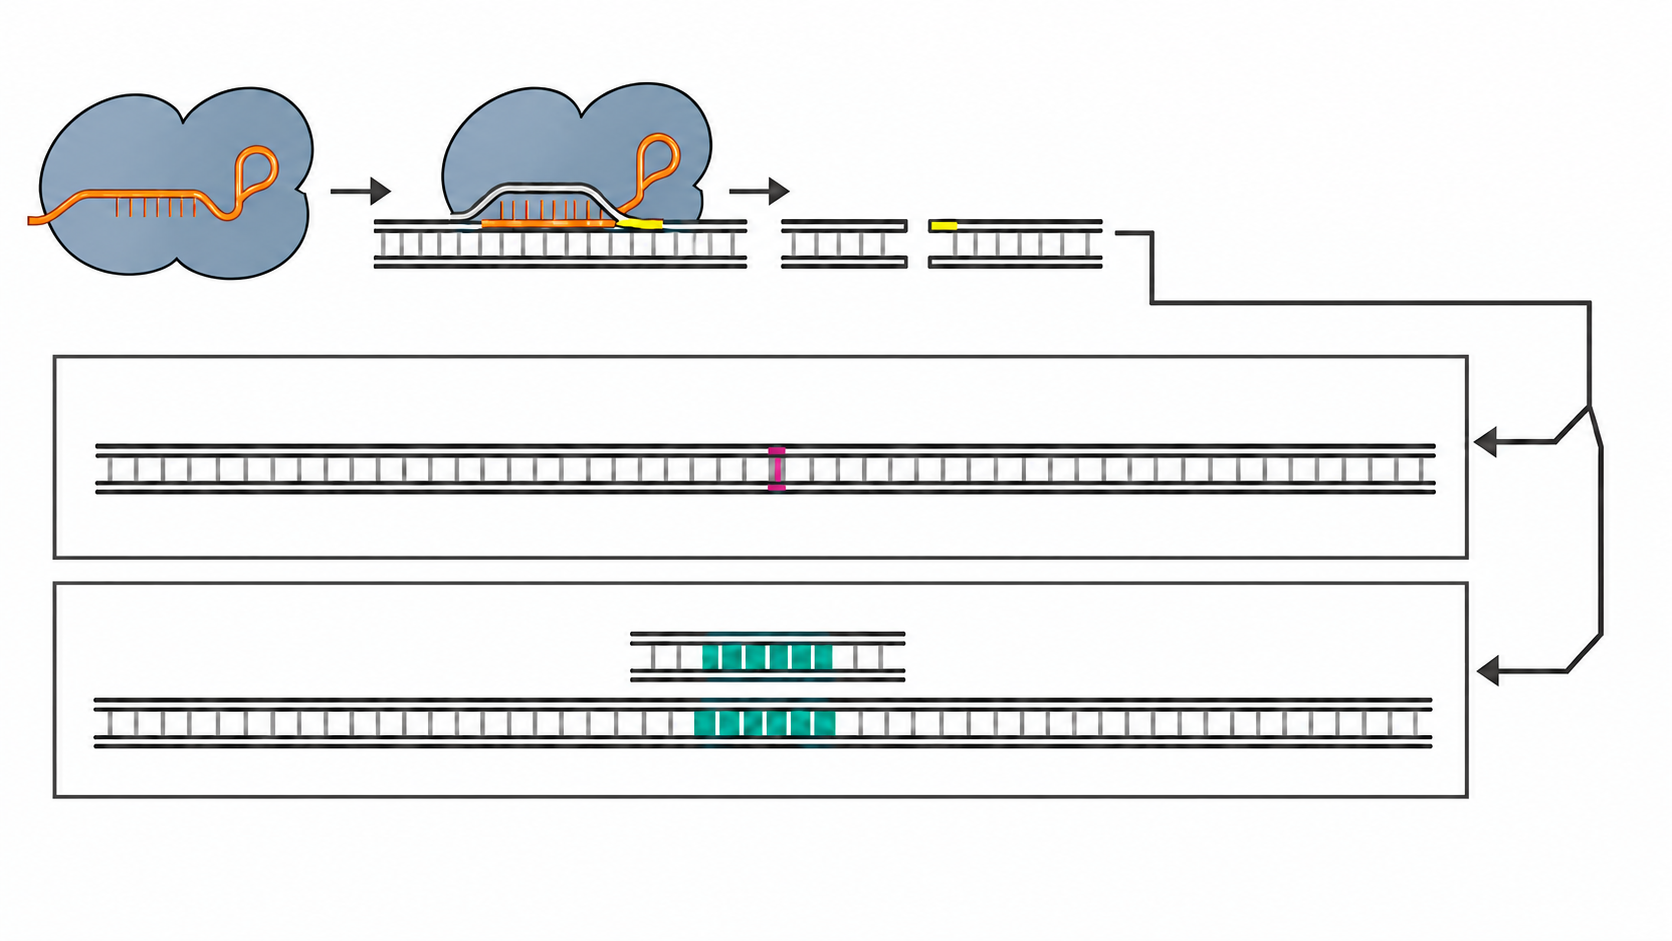
\includegraphics[width=\linewidth]{figures/ch03/ch03-06-final-base.png}};
  \begin{scope}[x={(img.south east)}, y={(img.north west)},
    lbl/.style={font=\sffamily\scriptsize, fill=white, fill opacity=0.88, text opacity=1, inner sep=1pt},
    ord/.style={circle, draw=orange!85!black, line width=0.5pt, fill=orange!15, inner sep=0.8pt, font=\sffamily\bfseries\tiny, text=BookInk}]
    \node[anchor=south west, inner sep=0, fill=white, fill opacity=0.92, text opacity=1] at (0.64,0.60) {%
      \resizebox{0.35\linewidth}{!}{% FIG ch03-07 PAM inset (English)
\begin{tikzpicture}[
  x=1mm, y=1mm,
  font=\sffamily\scriptsize,
  text=BookInk,
]
  \node[anchor=east] at (-2, 21.2) {Non-target strand};
  \node[anchor=east] at (-2, 7.2) {Target strand};
  \node at (6, 23.6) {5$'$};
  \node at (54.5, 23.6) {3$'$};
  \node at (55.5, 4.4) {5$'$};
  \node at (6, 4.4) {3$'$};

  \foreach \i in {0,...,19} {
    \pgfmathsetmacro{\x}{6+\i*2.4}
    \draw[draw=BookInk!50, fill=white] (\x,20) rectangle (\x+2.4,22.4);
  }
  \foreach \i in {0,1,2} {
    \pgfmathsetmacro{\x}{6+(17+\i)*2.4}
    \draw[draw=BookInk!50, fill=yellow!70] (\x,20) rectangle (\x+2.4,22.4);
  }
  \node[anchor=west, text=BookInk!80] at (6+17*2.4, 28.2) {PAM (NGG)};

  \foreach \i in {0,...,19} {
    \pgfmathsetmacro{\x}{6+\i*2.4}
    \draw[draw=BookInk!50, fill=white] (\x,6) rectangle (\x+2.4,8.4);
  }
  \foreach \i in {0,...,19} {
    \pgfmathsetmacro{\x}{6+\i*2.4}
    \draw[BookInk!35, thin] (\x+1.2,8.4) -- (\x+1.2,11.6);
    \draw[draw=orange!80!black, fill=orange!25, line width=1pt]
      (\x,4) rectangle (\x+2.4,6.4);
  }
  \draw[orange!80!black, line width=0.8pt]
    (6+19*2.4+2.4, 5) .. controls (6+21*2.4, 8) .. (6+21*2.4, 12)
    .. controls (6+21*2.4, 14) .. (6+19*2.4, 14);

  \node[anchor=west] at (6, 0.5) {sgRNA spacer};
  \pgfmathsetmacro{\cx}{6+16.5*2.4+1.2}
  \fill[black] (\cx,20) -- (\cx-0.8,21.2) -- (\cx+0.8,21.2) -- cycle;
  \fill[black] (\cx,6) -- (\cx-0.8,4.8) -- (\cx+0.8,4.8) -- cycle;
  \node[anchor=west] at (6+17.5*2.4, 13) {Cleavage site};
  \node[anchor=west, font=\scriptsize] at (6+16*2.4, 17) {RuvC};
  \node[anchor=west, font=\scriptsize] at (6+16*2.4, 3) {HNH};

  \draw[decorate, decoration={brace, amplitude=3pt}] (6, 15.5) -- (6+20*2.4, 15.5)
    node[midway, above=4pt] {$\sim$20 nt};
  \draw[decorate, decoration={brace, amplitude=2pt, mirror}] (6+16*2.4, 22.5) -- (6+17*2.4, 22.5)
    node[midway, below=2pt] {3 bp};
\end{tikzpicture}
}};
    \node[ord] at (0.04,0.92) {1};
    \node[ord] at (0.24,0.92) {2};
    \node[ord] at (0.46,0.82) {3};
    \node[ord] at (0.03,0.52) {4};
    \node[ord] at (0.03,0.22) {5};
    \node[lbl, font=\sffamily\bfseries\scriptsize] at (0.10,0.92) {Cas9};
    \node[lbl, font=\sffamily\bfseries\scriptsize] at (0.06,0.72) {sgRNA};
    \node[lbl] at (0.38,0.70) {PAM};
    \node[lbl] at (0.30,0.62) {Target DNA};
    \node[lbl] at (0.52,0.62) {Double-strand break};
    \node[lbl, anchor=west] at (0.06,0.48) {NHEJ (no template)};
    \node[lbl, anchor=west] at (0.06,0.22) {HDR (donor template)};
    \node[lbl] at (0.55,0.40) {Small indel};
    \node[lbl] at (0.50,0.34) {Donor template};
    \node[lbl] at (0.55,0.12) {Precise edit};
    \node[font=\sffamily\tiny, align=left, anchor=north west] at (0.02,0.04) {%
      Legend: solid arrow = step; split arrow = alternative repair routes; yellow = PAM; reddish-purple = indel; teal = donor-derived sequence};
  \end{scope}
\end{tikzpicture}
\caption{Final CRISPR--Cas9 genome editing overview figure. The text-free base image is combined with vector labels, a bottom legend bar, and the deterministic PAM detail inset (Figure~\ref{fig:ch03-07}) in the upper-right corner. The complete publication legend appears in the main text.}\label{fig:ch03-06}
\end{figure}

When drafting the figure legend—including with the \scidraw{} figure legend assistant (\sdtool{figure-legend})—verify every simplification statement and citation, and never invent efficiency percentages, sample sizes (\texttt{n=}), or statistical claims:

\begin{BookNote}
\textbf{Figure 1 | Overview of CRISPR--Cas9 genome editing and its two main repair outcomes.} A single guide RNA (sgRNA) binds Cas9. The complex recognizes a protospacer-adjacent motif (PAM; $5'$-NGG-$3'$ for SpCas9) in genomic DNA, the $\sim$20-nt spacer of the sgRNA base-pairs with the target strand, and Cas9 cleaves both strands about 3 bp upstream of the PAM, creating a double-strand break. The break can be repaired by non-homologous end joining (NHEJ), which needs no template and may leave small insertions or deletions (indels) that can disrupt a coding sequence; when a donor template with homology arms is supplied, homology-directed repair (HDR) can instead copy a precise change from the template. In most cell types HDR is less frequent than NHEJ. The inset shows the positions of the PAM, the target and non-target strands, and the cleavage site. For clarity, the three-dimensional structure of Cas9, the division of labor between the HNH and RuvC domains (except in the inset), repair factors, alternative end-joining pathways, off-target cleavage, and delivery methods are omitted. Based on Jinek et al.\ (2012), Doudna and Charpentier (2014), and Hsu et al.\ (2014).
\end{BookNote}

Finally, we verify Figure~\ref{fig:ch03-06} item by item against relationships C1--C9 (Table~\ref{tab:ch03-04-verify}).

\begin{table}[htbp]\centering\footnotesize
\setlength{\tabcolsep}{3pt}
\renewcommand{\arraystretch}{1.15}
\caption{Final verification record for the CRISPR--Cas9 overview figure.}\label{tab:ch03-04-verify}
\begin{tabularx}{\linewidth}{@{}l>{\raggedright\arraybackslash}p{22mm}>{\raggedright\arraybackslash}p{32mm}cY@{}}
\toprule
\textbf{\#} & \textbf{Relationship} & \textbf{Expected Visual Evidence} & \textbf{Status} & \textbf{Verification Notes} \\
\midrule
C1 & sgRNA--Cas9 binding & Both contact in Step 1 & Pass & Orange sgRNA contacts blue-gray Cas9; hairpin visible \\
C2 & PAM recognition & Complex at yellow PAM in Step 2 & Pass & Complex sits adjacent to bright-yellow PAM segment \\
C3 & Spacer--target pairing & RNA parallel to one strand, other displaced & Partial & Base image shows displaced arch, though rungs leave paired strand slightly schematic; clarified by upper-right TikZ inset \\
C4 & PAM position & Yellow block on non-target strand at $3'$ end & Pass & Base image keeps single right yellow block; inset locks exact $5'$-NGG-$3'$ polarity on non-target strand \\
C5 & Double-strand break & Both strands cut adjacent to PAM & Pass & Clean gap cuts both strands; $\sim$3 bp distance and HNH/RuvC assignment shown in inset \\
C6/C7 & NHEJ outcome & No template; reddish-purple indel mark & Pass & Upper lane 4 has no donor and a single central reddish-purple mark; legend uses ``may'' \\
C8/C9 & HDR outcome & Donor only here; DNA has teal insert & Partial & Lower lane 5 has sole short donor above teal insert (schematic length match) \\
--- & Reading order & Path 1--5 matches expected sequence & Pass & Top row 1--3 forks into lanes 4--5; DNA endpoint error 0.22\% (confirm with colleague blind test before submission) \\
--- & Exclusions & No nucleus, scissors, glow, or base text & Pass & 200\% zoom check confirms no baked-in text or forbidden objects \\
--- & Peer sign-off & Review by genome-editing colleague & Pending & Obtain colleague sign-off on inset strand polarity, HNH/RuvC labels, and legend phrasing before submission \\
\bottomrule
\end{tabularx}
\end{table}

Reviewing the workflow, the archived deliverables include: three sketches, three candidates with deviation notes, the comparison table and selection rationale, single-goal edit prompts and unrequested-change log, the deterministic inset, the text-free base image and final composite, the legend, and the verification record.

\section{What AI Can and Cannot Do at This Stage}

Table~\ref{tab:ch03-01} summarizes the boundaries between AI capabilities and author responsibilities during layout and sketch iteration.

\begin{table}[htbp]\centering\footnotesize
\setlength{\tabcolsep}{3pt}
\renewcommand{\arraystretch}{1.15}
\caption{What AI can do, what it cannot reliably do, and what the author must verify during layout and sketch development.}\label{tab:ch03-01}
\begin{tabularx}{\linewidth}{@{}>{\raggedright\arraybackslash}p{22mm}YYY@{}}
\toprule
\textbf{Sub-stage} & \textbf{What AI Can Do} & \textbf{What AI Cannot Do / Is Unreliable At} & \textbf{What the Author Must Verify} \\
\midrule
Proposing layout skeletons & Conversational AI can suggest verbal layout concepts and reading paths from a brief & Cannot judge which layout best fits the paper; \scidraw{} batch outputs share one prompt prior with limited structural variety & Draw at least one skeleton yourself; ensure all three skeletons differ in structure \\
Sketch $\rightarrow$ candidate figure & \scidraw{} Sketch Mode combines a sketch and prompt to quickly produce candidates following rough zones & A sketch is not a layout lock: objects may drift, merge, vanish, duplicate, or swap identities & Check each candidate against its sketch for position, direction, and count; log deviations \\
Evaluating reading order & A vision-capable conversational AI can describe where it would look first as an extra perspective & Model descriptions do not equal human eye paths and cannot replace peer testing & Have at least one colleague unfamiliar with the brief number the reading order \\
Choosing a layout & Can organize evaluation criteria into a comparison table & Cannot decide what the primary message of the figure should be & State the main message in the brief; record the selection rationale in the log \\
Iterative revision & Reference-image editing can adjust positions, delete objects, or resize frames per instruction & Local edits can cause collateral changes; outputs vary across runs; cannot enforce exact strand polarity or base distance & One goal per edit; overlay-compare with previous version; log unrequested changes; use TikZ for exact geometry \\
Scientific accuracy & Draws schematic relationships from prompts & Will not catch a PAM on the wrong strand, a distant cut site, or swapped NHEJ/HDR markers & Verify C1--C9 item by item; obtain domain-peer review \\
Text and labels & --- (base image must be text-free) & Generated text often misspells or misaligns terms & Overlay labels in LaTeX/TikZ and proofread spelling and positions \\
\bottomrule
\end{tabularx}
\end{table}

\section{Chapter Checklist}

\begin{itemize}
\item I can state the figure's entry point, path, and endpoint in one sentence.
\item The figure has only one visually heaviest element, and it carries the main message.
\item Objects grouped together (by proximity, alignment, or enclosure) are genuinely related; unrelated objects are not accidentally grouped.
\item At branch points, parallel options are drawn as parallel lanes so readers do not mistake them for sequential steps.
\item Details requiring exact geometry (strand polarity, position, base-pair distance) are drawn with deterministic tools or placed in an inset.
\item I drew and saved at least three structurally distinct sketches.
\item When generating candidates, I changed only the sketch while keeping the core brief text identical.
\item I checked each candidate against its sketch and logged positional deviations.
\item The reading order was tested by at least one person who had not seen the brief.
\item My layout choice is written as verifiable criteria rather than ``looks nicer.''
\item Every edit instruction has only one goal and states what must remain unchanged.
\item After each edit, I filled in the unrequested-change log and saved intermediate versions.
\item The final base image has no text; labels and legends are overlaid in LaTeX and checked for font size at final print width.
\end{itemize}

\section{Exercises}

\begin{enumerate}
\item \textbf{(Paper and pencil: Find the entry point of a figure)} Pick an overview figure or graphical abstract from a recent paper in your field. (a) Without reading the legend, look at the figure for 5 seconds and write down the first, second, and third elements you saw; (b) ask a classmate to do the same independently; (c) compare your sequences and identify which cues (size, contrast, position, arrows, numbering) caused agreement or divergence; (d) on a printout, sketch a better eye path and state which two elements should be moved.
\item \textbf{(Hands-on with \scidraw{}: One brief, three sketches)} Choose a process involving a branch or comparison (e.g., two failure modes of a material, or two branches of an algorithm). (a) Write a relationship table and drawing brief; (b) hand-draw linear, hub, and two-branch sketches and photograph them; (c) in \scidraw{} Sketch Mode, upload each sketch with the exact same brief text to generate candidates; (d) log deviations against the sketches and ask a classmate to number the reading order on all three; (e) score them with this chapter's comparison table and write your selection rationale. Submit: three sketches, three candidates, deviation log, and comparison table.
\item \textbf{(Revision discipline: From bundled feedback to single goals)} Here is a typical critique: ``Make the whole diagram cleaner, put the PAM in the right place, align the two outcomes, and make the colors more harmonious.'' (a) Split this into single-goal instructions, each stating what stays unchanged and how to check it; (b) point out which item should not be given to an image model, how to handle it instead, and why; (c) if you have candidates from Exercise 2, apply your instructions one by one, fill out the unrequested-change log, and count how many edits caused unrequested changes.
\end{enumerate}

\section*{References}

{\sloppy
\begin{itemize}
\item Chang HHY, Pannunzio NR, Adachi N, Lieber MR. Non-homologous DNA end joining and alternative pathways to double-strand break repair. \emph{Nature Reviews Molecular Cell Biology}. 2017;18(8):495--506. \path{doi:10.1038/nrm.2017.48}
\item Doudna JA, Charpentier E. The new frontier of genome engineering with CRISPR-Cas9. \emph{Science}. 2014;346(6213):1258096. \path{doi:10.1126/science.1258096}
\item Hsu PD, Lander ES, Zhang F. Development and applications of CRISPR-Cas9 for genome engineering. \emph{Cell}. 2014;157(6):1262--1278. \path{doi:10.1016/j.cell.2014.05.010}
\item Jinek M, Chylinski K, Fonfara I, Hauer M, Doudna JA, Charpentier E. A programmable dual-RNA--guided DNA endonuclease in adaptive bacterial immunity. \emph{Science}. 2012;337(6096):816--821. \path{doi:10.1126/science.1225829}
\item Nishimasu H, Ran FA, Hsu PD, Konermann S, Shehata SI, Dohmae N, Ishitani R, Zhang F, Nureki O. Crystal structure of Cas9 in complex with guide RNA and target DNA. \emph{Cell}. 2014;156(5):935--949. \path{doi:10.1016/j.cell.2014.02.001}
\item Ran FA, Hsu PD, Wright J, Agarwala V, Scott DA, Zhang F. Genome engineering using the CRISPR-Cas9 system. \emph{Nature Protocols}. 2013;8(11):2281--2308. \path{doi:10.1038/nprot.2013.143}
\item Rougier NP, Droettboom M, Bourne PE. Ten simple rules for better figures. \emph{PLoS Computational Biology}. 2014;10(9):e1003833. \path{doi:10.1371/journal.pcbi.1003833}
\item Wong B. Gestalt principles (Part 1). \emph{Nature Methods}. 2010a;7(11):863. \path{doi:10.1038/nmeth1110-863}
\item Wong B. Gestalt principles (Part 2). \emph{Nature Methods}. 2010b;7(12):941. \path{doi:10.1038/nmeth1210-941}
\item Wong B. Negative space. \emph{Nature Methods}. 2011b;8(1):5. \path{doi:10.1038/nmeth0111-5}
\item Wong B. Points of view: The overview figure. \emph{Nature Methods}. 2011c;8(5):365. \path{doi:10.1038/nmeth0511-365}
\item Wong B. Simplify to clarify. \emph{Nature Methods}. 2011d;8(8):611. \path{doi:10.1038/nmeth.1660}
\end{itemize}
\par}
